\newpage
\section{Support Vector Machines: Maximum-Margin Classification and Kernel Methods}
\label{sec:support-vector-machines}

This section evaluates support vector machines (SVMs) for churn prediction. The previous sections considered probability-based linear classifiers, nearest-neighbour methods, probabilistic models, individual decision trees, bagging, random forests, and boosting. SVMs provide a distinct modelling principle. Rather than estimating a conditional probability directly, an SVM constructs a decision boundary and seeks a boundary with a large separation margin between the two classes.

The held-out test set is not used in this section. All tuning, selection, figures, tables, and comparisons are based on stratified cross-validation within the training set. The reported configurations are therefore development-stage candidates selected within transparent fixed grids. They are not final globally optimized models and they do not provide final held-out test performance.

\subsection{Linear decision scores and separating hyperplanes}

For a binary classification problem, a linear SVM starts with the score
\[
f(x) = w^\top x + b,
\]
where \(x\) is the transformed feature vector, \(w\) is the coefficient vector, and \(b\) is an intercept. The decision boundary is the hyperplane
\[
w^\top x + b = 0.
\]
For labels coded as \(y_i \in \{-1,+1\}\), the sign of the score determines the predicted class:
\[
\widehat{y}_i = \operatorname{sign}(f(x_i)).
\]

The numerical value of \(f(x)\) is a signed decision score. A large positive score places an observation on the positive-class side of the boundary, while a large negative score places it on the negative-class side. Unlike logistic regression, the raw score is not a calibrated probability. This distinction is important later when interpreting score thresholds.

\subsection{Maximum margin and support vectors}

A separating hyperplane is not unique when the classes can be separated. SVMs select a separator by maximizing the margin, namely the distance between the boundary and the closest training observations. Under the conventional scaling of the score, the two margin boundaries are
\[
w^\top x + b = +1
\qquad \text{and} \qquad
w^\top x + b = -1.
\]
Their distance is
\[
\frac{2}{\lVert w \rVert}.
\]

For perfectly separable data, the hard-margin SVM solves
\[
\min_{w,b} \frac{1}{2}\lVert w \rVert^2
\]
subject to
\[
y_i(w^\top x_i+b)\geq 1,
\qquad i=1,\ldots,n.
\]
Minimizing \(\lVert w\rVert^2\) maximizes the margin. The observations that lie on the margin, or violate it in the nonseparable case, are the \emph{support vectors}. They determine the fitted boundary most directly.

Hard-margin separation is usually too restrictive for real churn data. Classes overlap, predictors contain noise, and some customer profiles are difficult to classify. The practical model is therefore the soft-margin SVM.

\subsection{Soft margins, hinge loss, and regularization}

The soft-margin SVM introduces non-negative slack variables \(\xi_i\):
\[
\min_{w,b,\xi}
\frac{1}{2}\lVert w\rVert^2
+
C\sum_{i=1}^{n}\xi_i
\]
subject to
\[
y_i(w^\top x_i+b)\geq 1-\xi_i,
\qquad
\xi_i\geq 0.
\]
The parameter \(C>0\) controls the tradeoff between a wide, regularized margin and penalties for observations that lie inside the margin or on the wrong side of the boundary. Smaller \(C\) values impose stronger regularization and tolerate more margin violations. Larger \(C\) values penalize violations more strongly and can create a more flexible, higher-variance boundary.

The same principle can be written through hinge loss:
\[
\ell_{\mathrm{hinge}}(y_i,f(x_i))
=
\max\{0,1-y_i f(x_i)\}.
\]
The corresponding unconstrained objective is
\[
\min_{w,b}
\frac{1}{2}\lVert w\rVert^2
+
C\sum_{i=1}^{n}
\max\{0,1-y_i f(x_i)\}.
\]

The notebook evaluates both the standard hinge loss and the squared-hinge variant exposed by \texttt{LinearSVC}:
\[
\ell_{\mathrm{squared\ hinge}}(y_i,f(x_i))
=
\left[
\max\{0,1-y_i f(x_i)\}
\right]^2.
\]
Both losses encourage correct classification with margin. The squared-hinge loss penalizes large margin violations more strongly and is the default loss used by scikit-learn's linear SVM implementation.

\subsection{Class weighting for imbalanced churn detection}

Churn is the minority class in the training data. A class-weighted SVM changes the loss penalty by class:
\[
\min_{w,b}
\frac{1}{2}\lVert w\rVert^2
+
C\sum_{i=1}^{n}
c_{y_i}\,
\max\{0,1-y_i f(x_i)\},
\]
where \(c_{y_i}\) is a class-specific weight. The \texttt{balanced} option increases the effective penalty for misclassifying churners relative to non-churners. This does not necessarily improve the quality of the score ranking. Instead, it can shift the natural zero-score decision boundary toward higher recall and a larger fraction of customers flagged as potential churners.

\subsection{Kernel SVMs}

A linear SVM uses the original transformed feature representation. A kernel SVM permits a nonlinear boundary by treating the classifier as linear in an implicit feature map \(\phi(x)\):
\[
f(x)
=
w^\top \phi(x) + b.
\]
The kernel trick avoids explicitly constructing \(\phi(x)\). Instead, it uses a kernel function
\[
K(x,z)=\phi(x)^\top\phi(z).
\]

In the dual representation, the fitted score can be expressed in terms of support vectors:
\[
f(x)
=
\sum_{i\in\mathcal{S}}
\alpha_i y_i K(x_i,x)
+
b,
\]
where \(\mathcal{S}\) contains the support vectors and \(\alpha_i\) are learned non-negative weights.

The primary nonlinear candidate in this section is the radial basis function (RBF) kernel:
\[
K(x,z)
=
\exp\left(-\gamma\lVert x-z\rVert^2\right).
\]
The parameter \(\gamma>0\) controls locality. Small \(\gamma\) values yield smoother, more global similarity regions. Large \(\gamma\) values create highly local decision regions and can increase variance. RBF SVMs therefore require careful joint interpretation of \(C\) and \(\gamma\).

\subsection{Leakage-safe preprocessing and evaluation design}

SVMs are not scale invariant. The workflow standardizes numeric variables and one-hot encodes categorical variables inside an sklearn pipeline. Each preprocessing object is fitted separately within each cross-validation training fold. Consequently, scaling means, scaling variances, imputation decisions, and one-hot category mappings are not learned from the validation fold.

The section uses the project-wide stratified cross-validation design and treats PR-AUC as the primary selection metric because churn is the positive minority class. ROC-AUC, balanced accuracy, precision, recall, specificity, and \(F_1\) are retained as secondary diagnostics. The linear and kernel SVM implementations use raw \texttt{decision\_function} scores for ranking metrics and curves. The kernel SVC does not enable \texttt{probability=True}; this avoids nesting an additional internal probability-fitting procedure inside each cross-validation fit.

\subsection{Kernel-family screen}

Before tuning the main linear and RBF grids, the notebook evaluates a compact kernel-family screen. Table~\ref{tab:svm-kernel-screen} reports pooled out-of-fold diagnostics. The squared-hinge linear SVM has the strongest PR-AUC in this initial screen, \(0.654\), closely followed by the RBF SVC at \(0.652\). The hinge-loss linear SVM, linear-kernel SVC, and quadratic polynomial SVC all remain in a narrow range between \(0.646\) and \(0.648\).

\begin{table}[H]
\centering
\small
\resizebox{\textwidth}{!}{
\begin{tabular}{lrrrrrrrr}
\toprule
Candidate & Accuracy & Bal. Acc. & Precision & Recall & Specificity & \(F_1\) & ROC-AUC & PR-AUC \\
\midrule
LinearSVC, squared hinge, \(C=1\) & 0.803 & 0.717 & 0.658 & 0.535 & 0.899 & 0.590 & 0.842 & 0.654 \\
RBF SVC, \(C=1,\gamma=0.01\) & 0.800 & 0.700 & 0.669 & 0.486 & 0.913 & 0.563 & 0.835 & 0.652 \\
LinearSVC, hinge, \(C=1\) & 0.799 & 0.714 & 0.647 & 0.534 & 0.895 & 0.585 & 0.834 & 0.648 \\
Linear-kernel SVC, \(C=1\) & 0.799 & 0.714 & 0.648 & 0.534 & 0.895 & 0.585 & 0.834 & 0.648 \\
Polynomial SVC, degree \(2\), \(C=1\) & 0.807 & 0.711 & 0.686 & 0.505 & 0.916 & 0.582 & 0.818 & 0.646 \\
\bottomrule
\end{tabular}
}
\caption{Kernel-family screen using pooled out-of-fold predictions on the training set}
\label{tab:svm-kernel-screen}
\end{table}

The screen does not show a material nonlinear advantage. In particular, the quadratic polynomial kernel does not improve ranking quality, and the RBF model is essentially tied with the strongest linear implementation. This is plausible for one-hot encoded tabular churn data: the representation already captures substantial categorical structure, while the remaining signal can be approximated well by an additive linear score.

The two linear implementations should be expected to be close but not exactly identical. \texttt{LinearSVC} and \texttt{SVC(kernel="linear")} use different solvers and implementation details. Their near-identical results nevertheless support the conclusion that the linear margin formulation is stable in this data setting.

\begin{figure}[H]
\centering
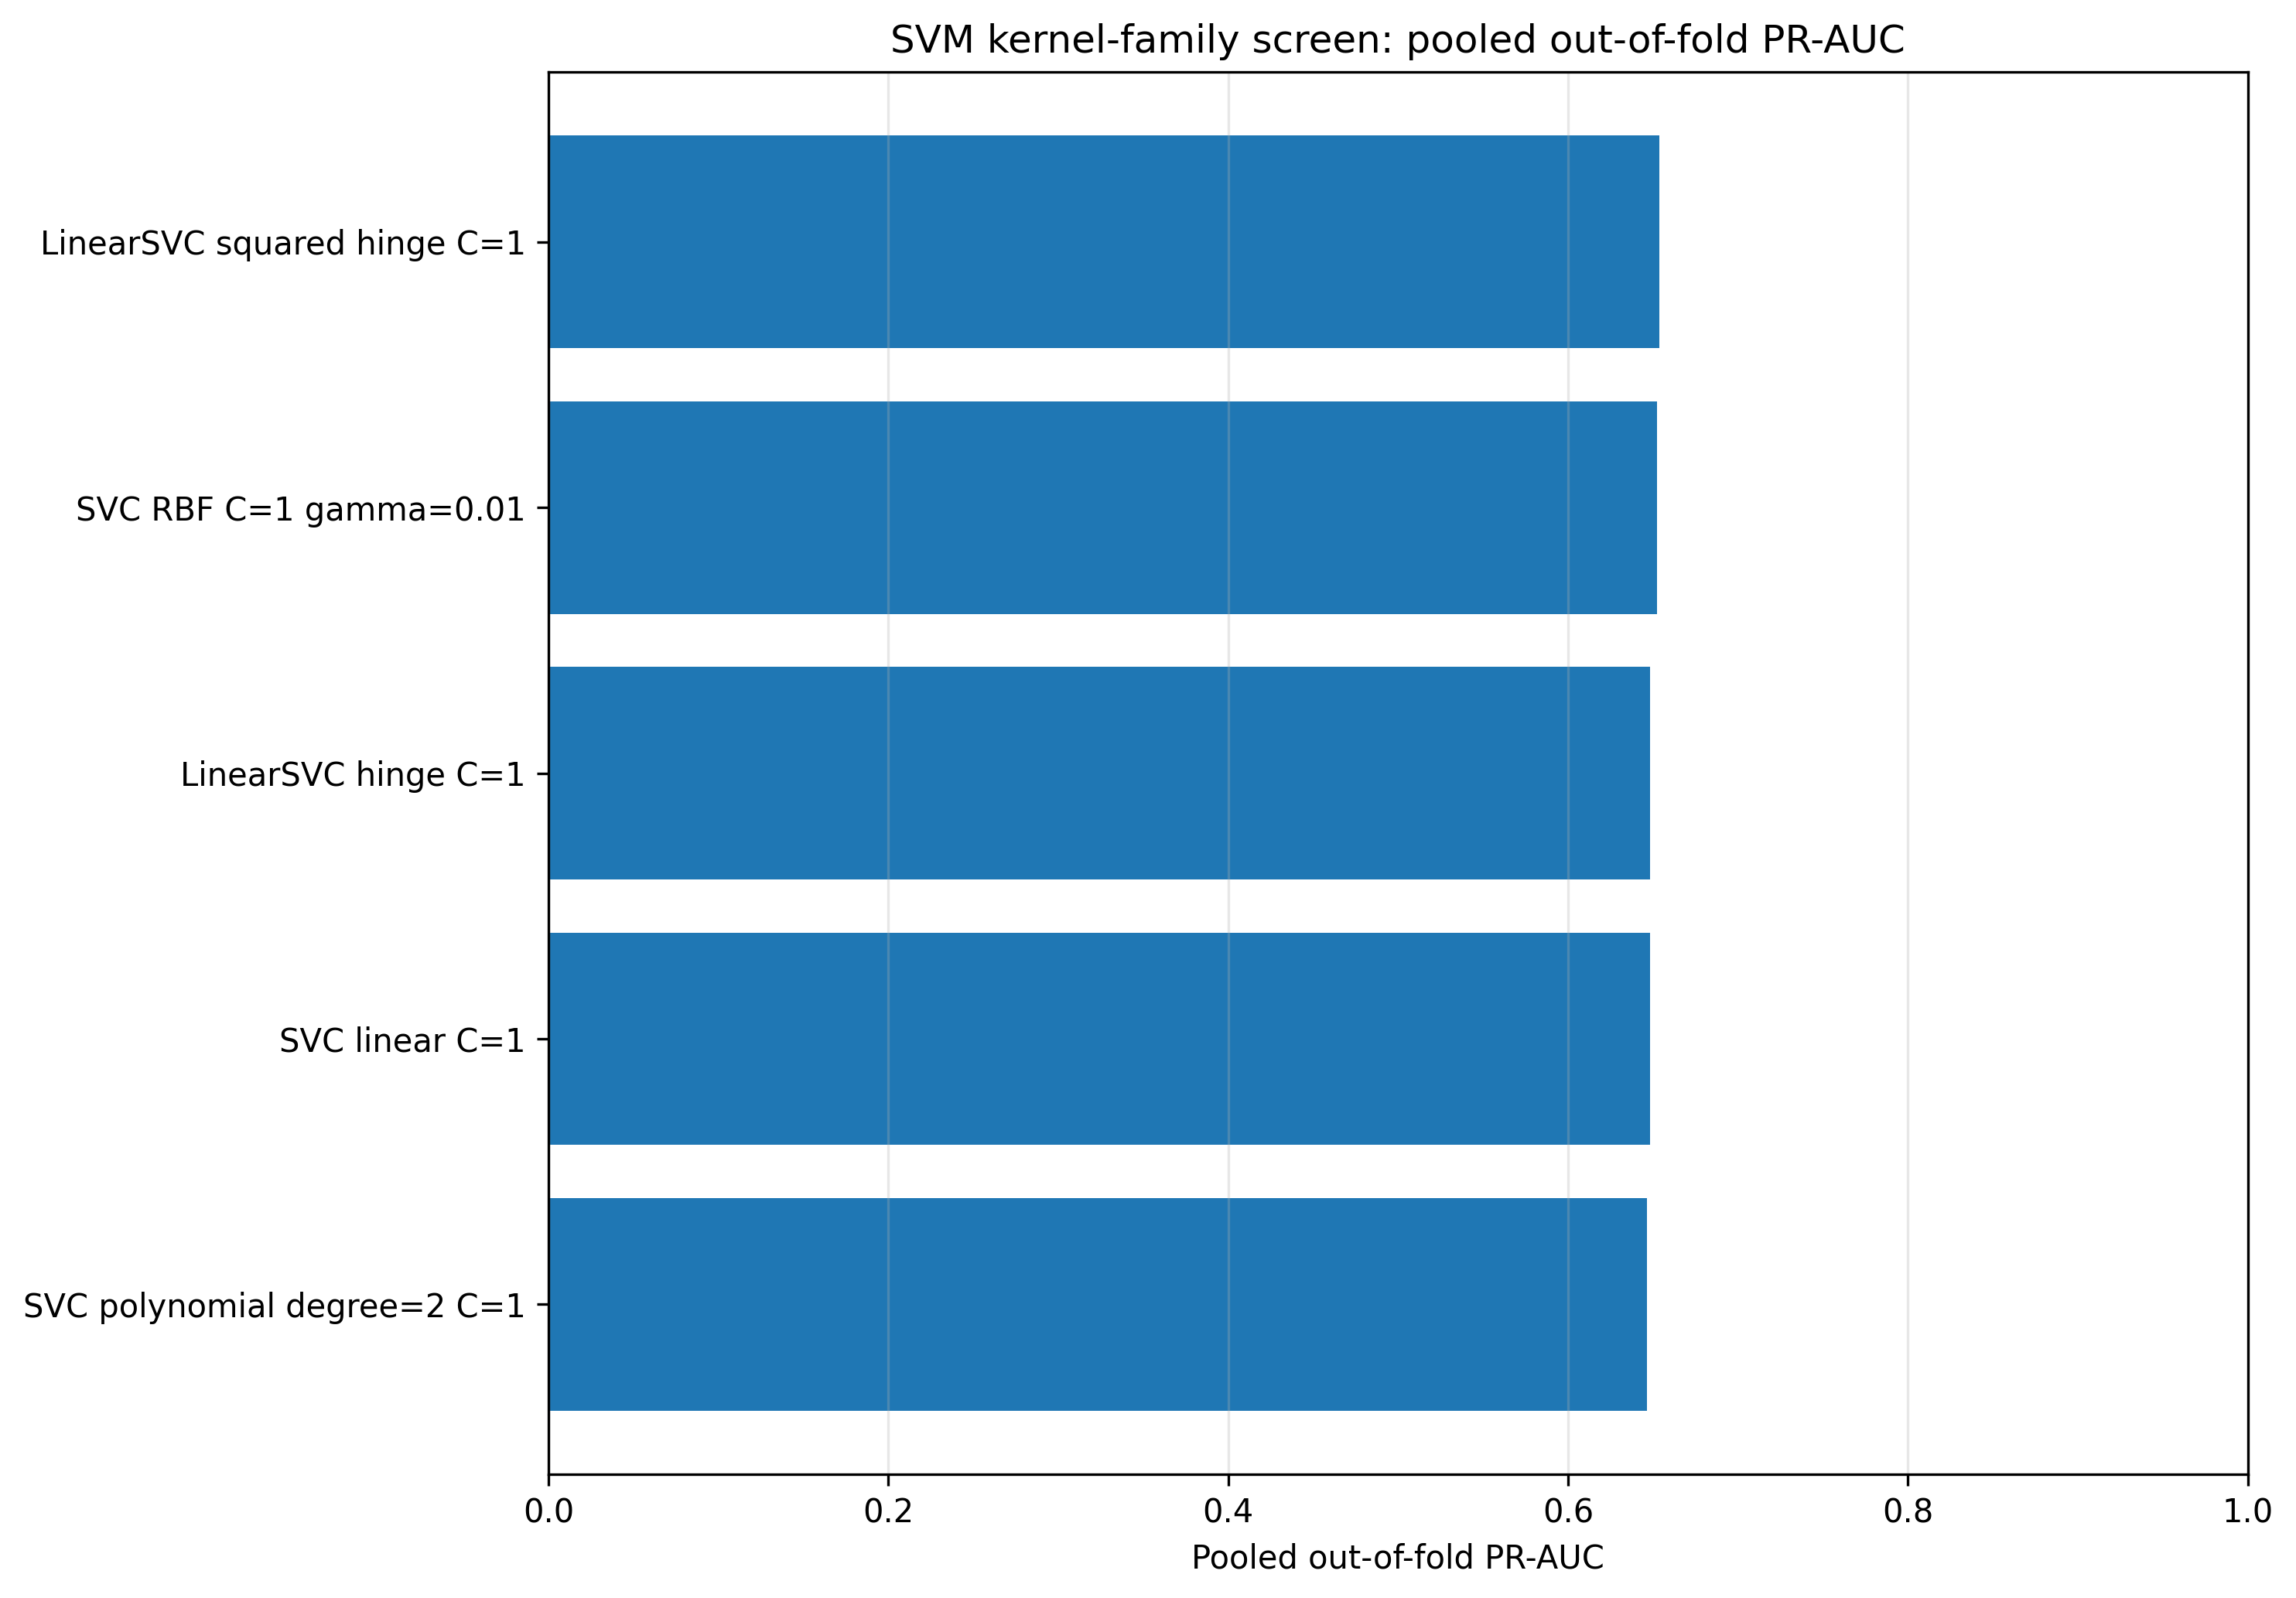
\includegraphics[width=0.88\textwidth]{../figures/svm_kernel_screen_pr_auc.png}
\caption{Kernel-family screen: pooled out-of-fold PR-AUC}
\label{fig:svm-kernel-screen}
\end{figure}

\subsection{Linear SVM fixed grid}

The linear SVM grid varies \(C\), loss function, and class weighting. Table~\ref{tab:svm-linear-grid-summary} presents representative rows from the fixed grid. The strongest observed linear configuration uses squared hinge loss, \(C=0.1\), and \texttt{class\_weight="balanced"}. Its mean fold-level validation PR-AUC is \(0.659\), with mean ROC-AUC \(0.845\), balanced accuracy \(0.765\), and \(F_1\) \(0.627\).

\begin{table}[H]
\centering
\small
\begin{tabular}{llrrrrr}
\toprule
Loss & Class weight & \(C\) & Mean CV PR-AUC & Mean CV ROC-AUC & Bal. Acc. & \(F_1\) \\
\midrule
Squared hinge & balanced & 0.10 & 0.659 & 0.845 & 0.765 & 0.627 \\
Squared hinge & none & 0.10 & 0.657 & 0.843 & 0.715 & 0.587 \\
Hinge & balanced & 0.01 & 0.658 & 0.842 & 0.751 & 0.606 \\
Hinge & none & 0.01 & 0.652 & 0.837 & 0.714 & 0.585 \\
\bottomrule
\end{tabular}
\caption{Representative linear-SVM fixed-grid results using mean fold-level validation metrics}
\label{tab:svm-linear-grid-summary}
\end{table}

The squared-hinge balanced candidates are stable across the tested \(C\) range. Their mean validation PR-AUC remains between approximately \(0.658\) and \(0.659\) for \(C\in\{0.01,0.1,1,10\}\). This is evidence that the linear SVM is not highly sensitive to the tested regularization range. It does not establish that exactly \(C=0.1\) is uniquely optimal.

Class weighting changes the default operating point more strongly than the ranking quality. At \(C=0.1\), enabling balanced weights raises mean recall from \(0.532\) to \(0.807\) and mean balanced accuracy from \(0.715\) to \(0.765\), while mean precision falls from \(0.655\) to \(0.513\). The class-weighted model identifies more potential churners at the natural score boundary, which can be attractive when missed churners are costly.

\begin{figure}[H]
\centering
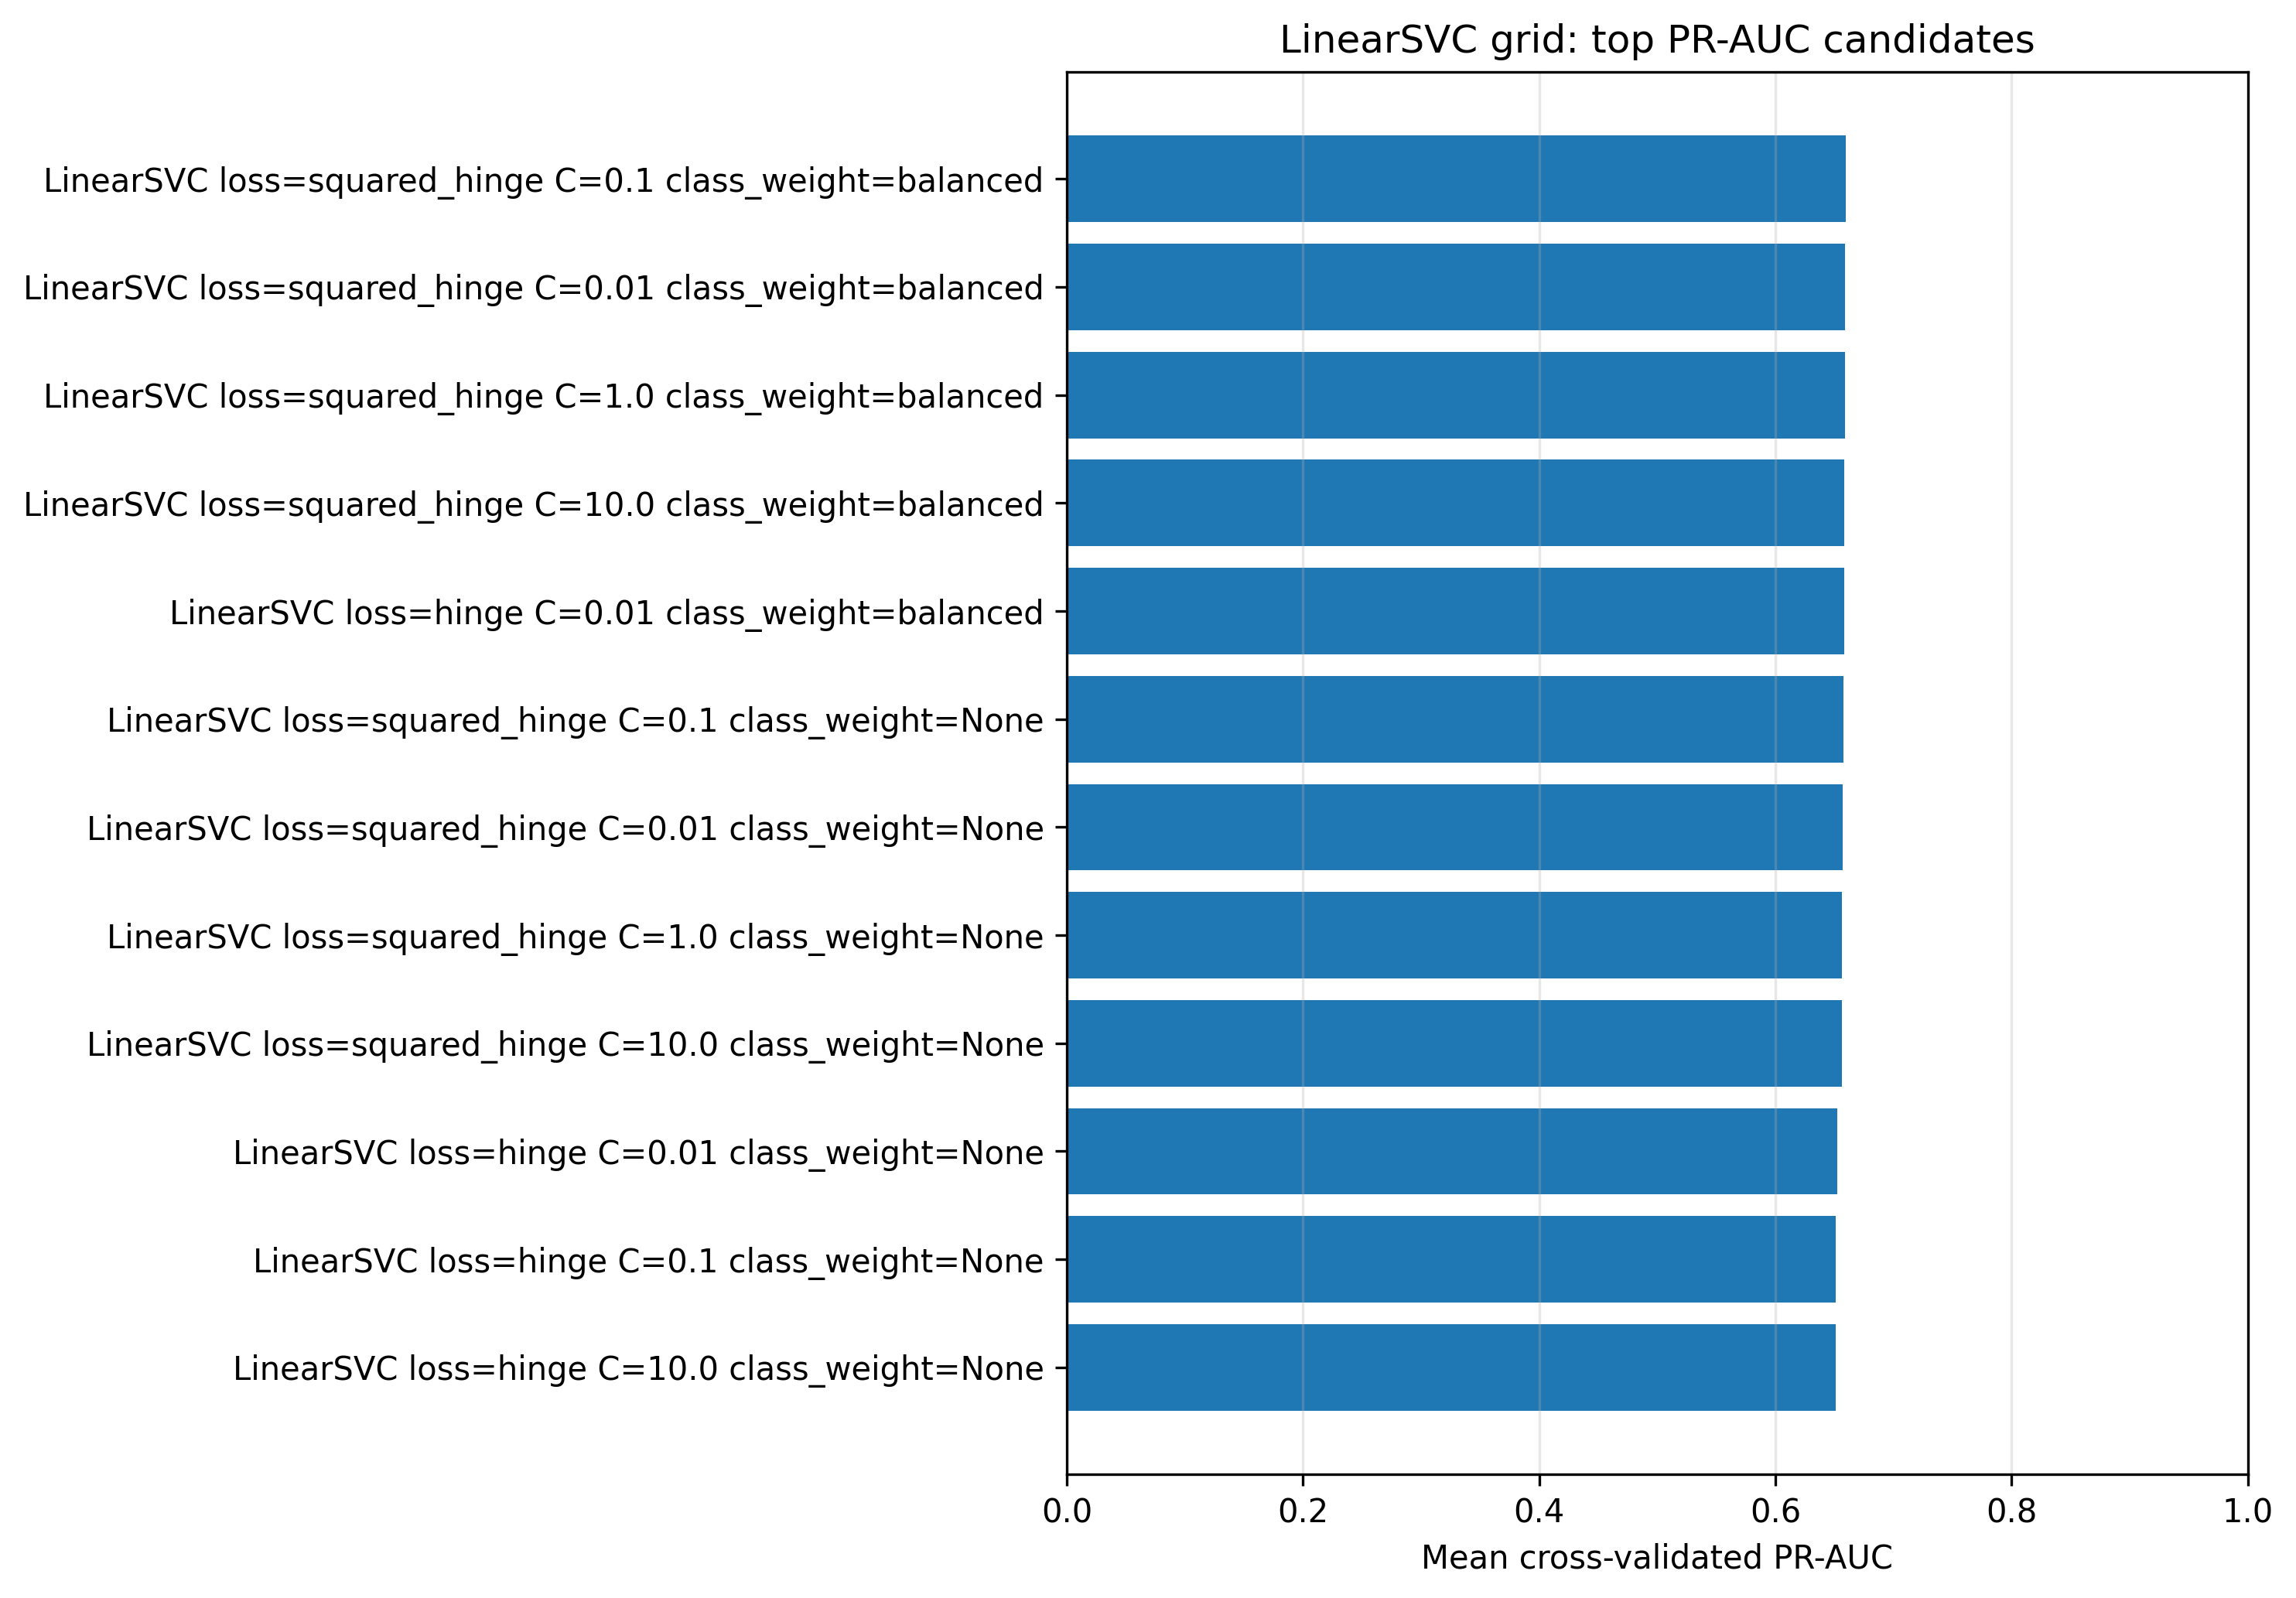
\includegraphics[width=0.88\textwidth]{../figures/svm_linear_grid_pr_auc.png}
\caption{LinearSVC fixed grid: top mean cross-validated PR-AUC candidates}
\label{fig:svm-linear-grid}
\end{figure}

\subsection{RBF-kernel SVM fixed grid}

The RBF grid varies \(C\), \(\gamma\), and class weighting. The strongest observed RBF candidate is
\[
C=10,
\qquad
\gamma=0.001,
\qquad
\texttt{class\_weight="balanced"}.
\]
Its mean fold-level validation PR-AUC is \(0.6595\), only \(0.0001\) above the strongest linear candidate. Table~\ref{tab:svm-rbf-grid-summary} shows representative configurations.

\begin{table}[H]
\centering
\small
\resizebox{\textwidth}{!}{%
\begin{tabular}{rrlrrrr}
\toprule
\(C\) & \(\gamma\) & Class weight & Mean CV PR-AUC & Mean CV ROC-AUC & Train PR-AUC & Fit time (s) \\
\midrule
10.0 & 0.001 & balanced & 0.659 & 0.842 & 0.663 & 0.419 \\
1.0 & 0.010 & balanced & 0.658 & 0.842 & 0.668 & 0.438 \\
0.1 & 0.010 & balanced & 0.655 & 0.840 & 0.657 & 0.442 \\
10.0 & 0.100 & none & 0.572 & 0.773 & 0.857 & 0.464 \\
\bottomrule
\end{tabular}%
}
\caption{Representative RBF-SVC fixed-grid results using mean fold-level validation metrics}
\label{tab:svm-rbf-grid-summary}
\end{table}

The small selected \(\gamma\) value corresponds to a smooth nonlinear boundary. The grid also shows the expected high-variance failure mode at large \(\gamma\). With \(C=10\), \(\gamma=0.1\), and no class weighting, mean training PR-AUC rises to \(0.857\) while mean validation PR-AUC falls to \(0.572\). This large train-validation gap indicates that a very local RBF boundary can fit fold-specific structure without improving unseen churn ranking.

The selected RBF candidate requires substantially more computation than the selected linear candidate. Mean per-fold fit time is approximately \(0.419\) seconds for the selected RBF SVC versus approximately \(0.039\) seconds for the selected LinearSVC. The difference is not prohibitive for this dataset, but it matters when the nonlinear model does not provide a clear ranking improvement.

\begin{figure}[H]
\centering
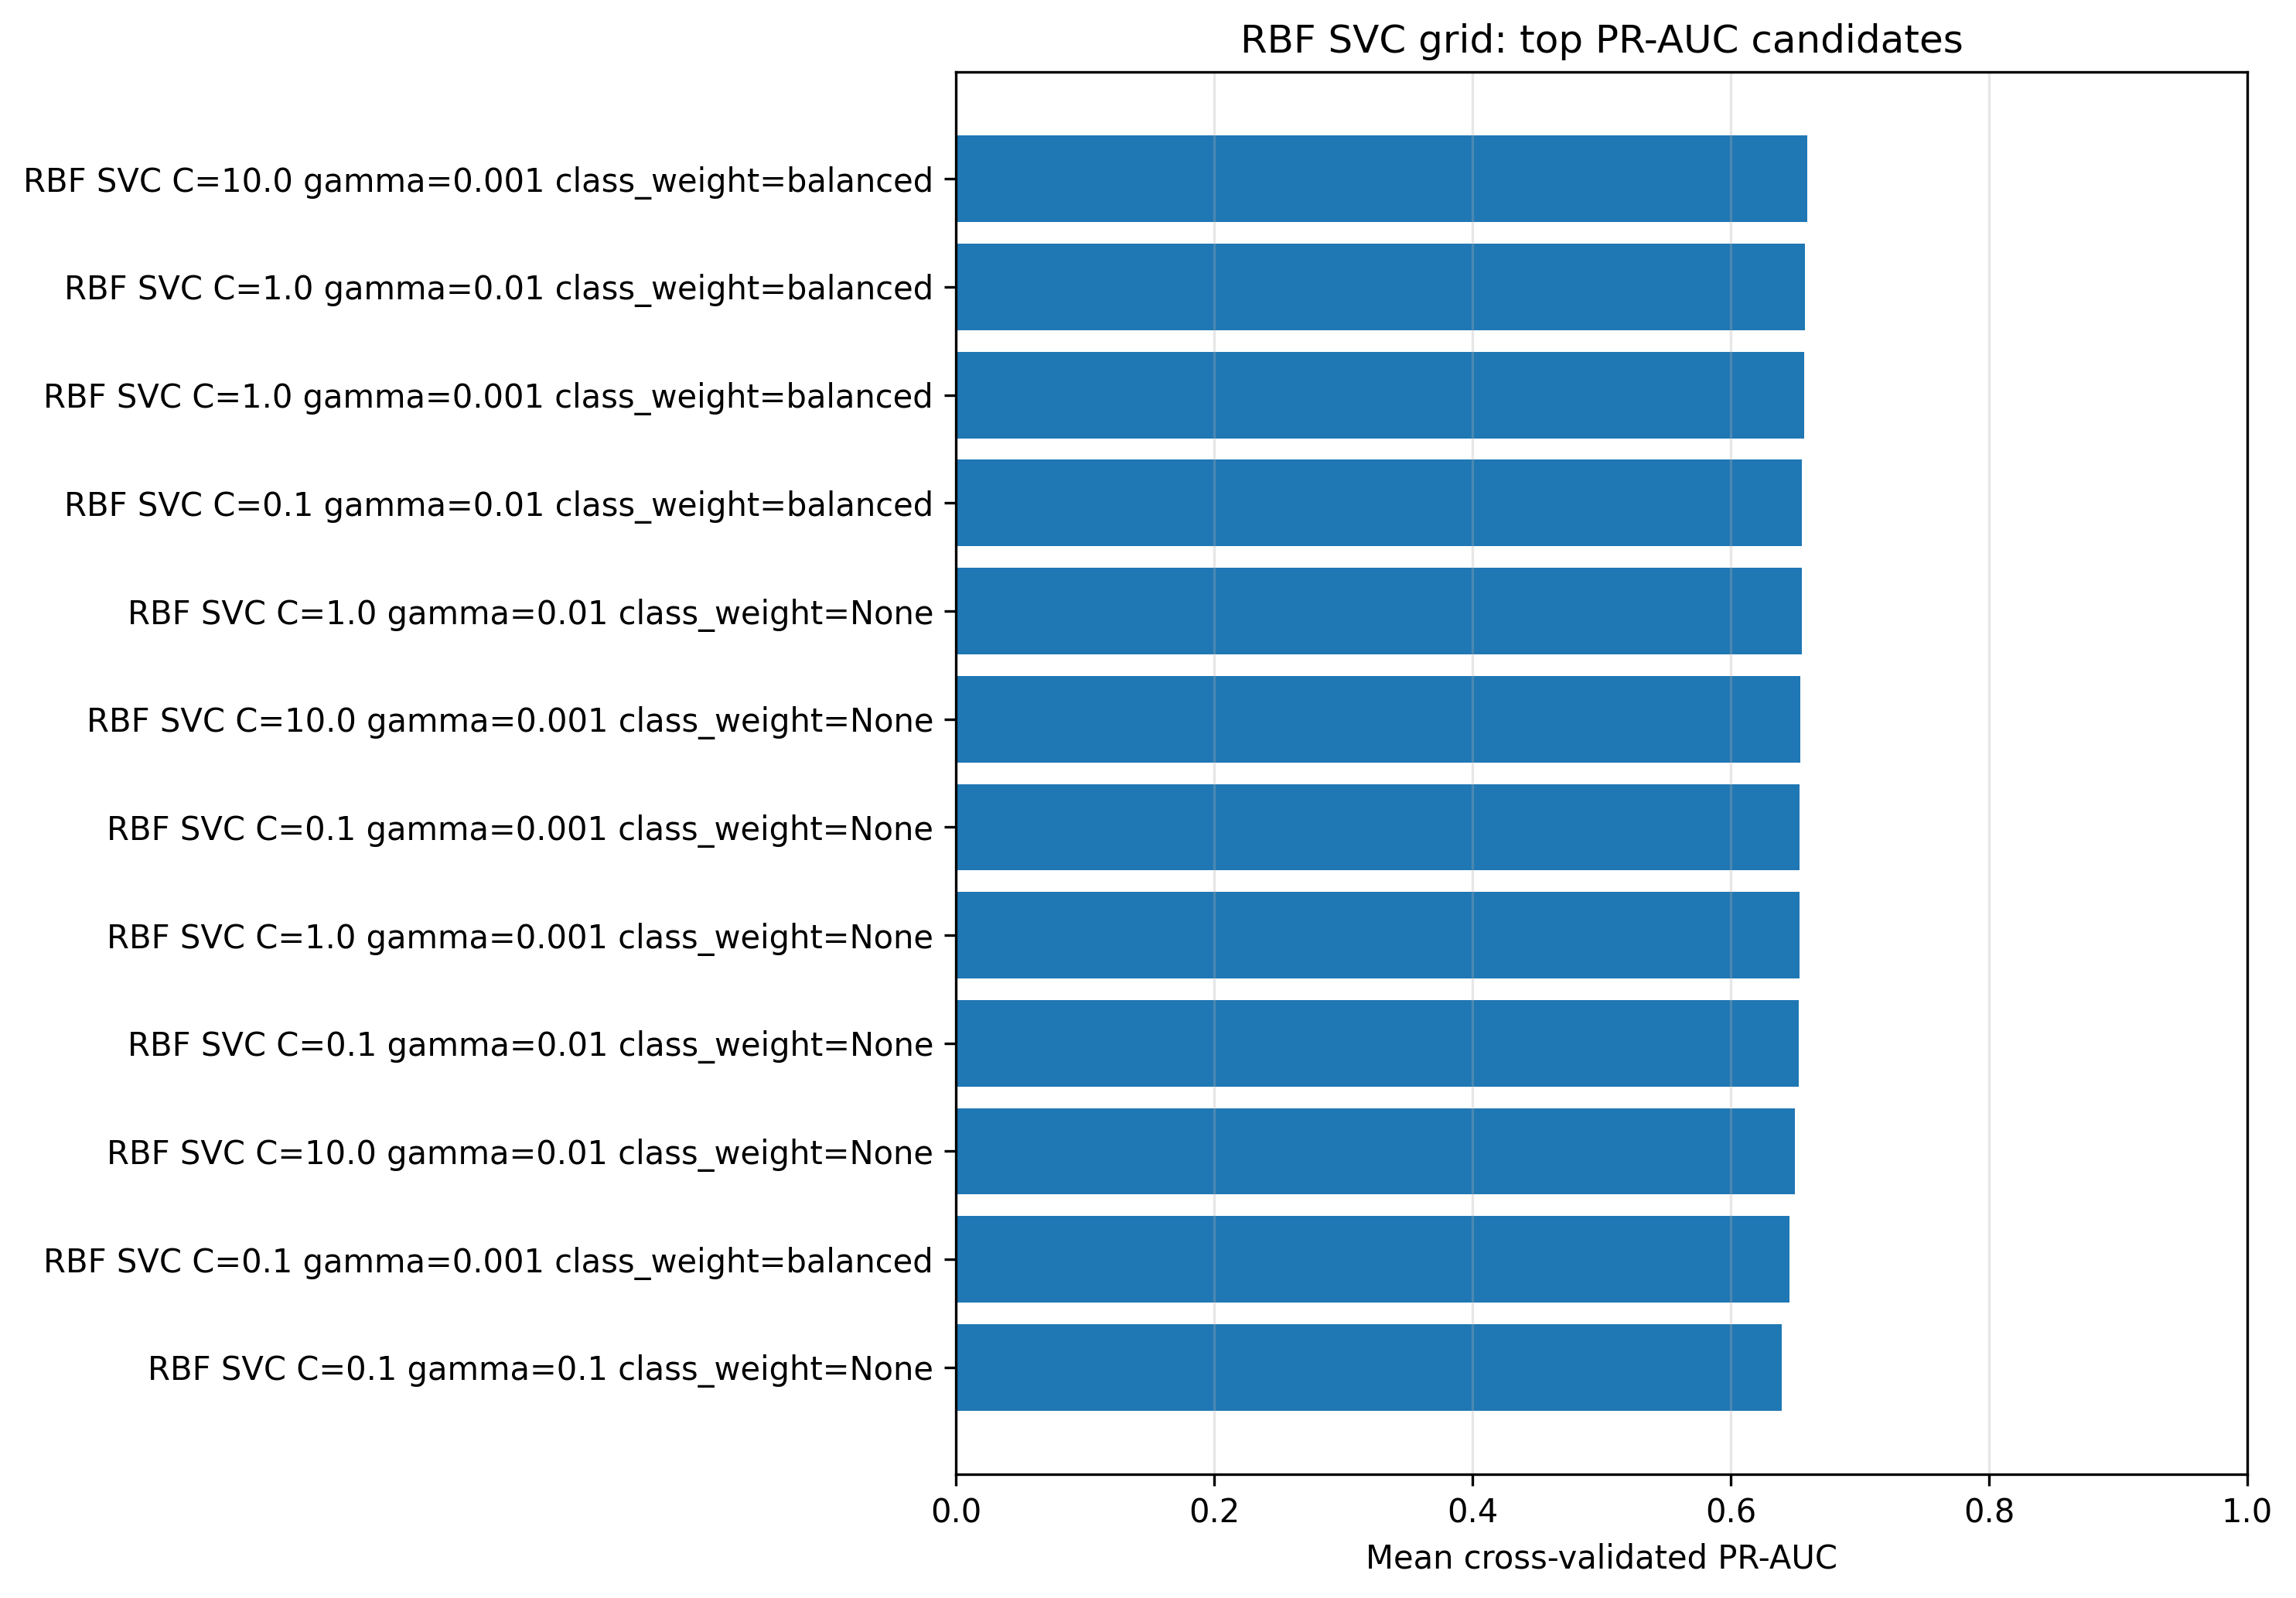
\includegraphics[width=0.88\textwidth]{../figures/svm_rbf_grid_pr_auc.png}
\caption{RBF-SVC fixed grid: top mean cross-validated PR-AUC candidates}
\label{fig:svm-rbf-grid}
\end{figure}

\subsection{Selected linear and RBF candidates}

Table~\ref{tab:svm-selected-family-candidates} summarizes the selected candidate from each SVM family. The fixed-grid family-selection rule is mean fold-level validation PR-AUC, followed by balanced accuracy and \(F_1\). The RBF candidate has a numerically larger PR-AUC by only \(0.0001\), far below the observed fold-to-fold standard deviations of \(0.016\) to \(0.018\). The appropriate conclusion is that the selected linear and RBF candidates are effectively tied within this development grid.

\begin{table}[H]
\centering
\small
\resizebox{\textwidth}{!}{%
\begin{tabular}{llrrrr}
\toprule
Family & Selected configuration & Mean CV PR-AUC & Mean CV ROC-AUC & Bal. Acc. & \(F_1\) \\
\midrule
LinearSVC & squared hinge, \(C=0.1\), balanced & 0.6594 & 0.8453 & 0.7648 & 0.6267 \\
RBF SVC & \(C=10\), \(\gamma=0.001\), balanced & 0.6595 & 0.8424 & 0.7464 & 0.6003 \\
\bottomrule
\end{tabular}%
}
\caption{Selected linear and RBF SVM candidates from the fixed development grids}
\label{tab:svm-selected-family-candidates}
\end{table}

The subsequent pooled out-of-fold diagnostic produces a different ordering. The selected linear model has pooled OOF PR-AUC \(0.6565\), whereas the selected RBF model has \(0.6426\). This is not a contradiction. Mean fold-level PR-AUC and PR-AUC calculated after concatenating all out-of-fold scores are different statistics. PR-AUC is nonlinear, and the raw decision-score scales of separately fitted SVMs can differ across folds. The pre-specified mean fold-level statistic remains the appropriate grid-selection criterion. The pooled diagnostic is used for descriptive curves, confusion matrices, and a common within-section comparison.

Taken together, the results justify retaining the linear SVM as the representative SVM for detailed diagnostics. It is essentially tied with RBF in the selected grid, is materially faster, yields directly interpretable coefficient directions, and has the stronger pooled OOF diagnostic. This does not prove that linear SVM is globally superior to RBF SVM.

\subsection{Scoped comparison with selected reference models}

For this section, the selected SVM candidates are compared with representative models from earlier sections. The earlier model rows are not copied from stored result CSV files. Each selected configuration is reconstructed from its previously selected hyperparameters and re-evaluated through fresh training-only cross-validation in the SVM notebook. This supplies comparable pooled out-of-fold predictions, metrics, and confusion matrices under the same current evaluation procedure.

The comparison is deliberately scoped. It includes logistic regression, kNN, a single tree, bagging, random forest, and a strong XGBoost reference. It does not include every selected boosting implementation, such as CatBoost, LightGBM, or \texttt{GradientBoostingClassifier}. Therefore, Table~\ref{tab:svm-model-comparison} is a section-level diagnostic, not the final project-wide model ranking.

\begin{table}[H]
\centering
\small
\resizebox{\textwidth}{!}{
\begin{tabular}{lrrrrrrrr}
\toprule
Model & Accuracy & Bal. Acc. & Precision & Recall & Specificity & \(F_1\) & ROC-AUC & PR-AUC \\
\midrule
Best XGBoost reference & 0.808 & 0.722 & 0.671 & 0.539 & 0.905 & 0.598 & 0.850 & 0.670 \\
Selected bagged trees & 0.800 & 0.705 & 0.662 & 0.504 & 0.907 & 0.572 & 0.846 & 0.662 \\
Selected random forest & 0.804 & 0.706 & 0.678 & 0.498 & 0.914 & 0.574 & 0.847 & 0.660 \\
Selected L2 logistic regression & 0.802 & 0.719 & 0.652 & 0.544 & 0.895 & 0.593 & 0.846 & 0.658 \\
Selected LinearSVC & 0.745 & 0.765 & 0.513 & 0.807 & 0.723 & 0.627 & 0.845 & 0.657 \\
Selected RBF SVC & 0.706 & 0.746 & 0.469 & 0.833 & 0.659 & 0.600 & 0.838 & 0.643 \\
Selected single decision tree & 0.789 & 0.701 & 0.624 & 0.514 & 0.888 & 0.564 & 0.824 & 0.628 \\
Selected kNN & 0.792 & 0.722 & 0.617 & 0.571 & 0.872 & 0.593 & 0.836 & 0.628 \\
\bottomrule
\end{tabular}
}
\caption{Scoped pooled out-of-fold comparison of selected SVMs and reconstructed reference models}
\label{tab:svm-model-comparison}
\end{table}

The selected linear SVM is competitive with L2 logistic regression, bagging, and random forests in ranking performance, but it does not surpass the strong XGBoost reference in this scoped comparison. Its default operating point is notably less conservative. It detects many more churners, but also flags more non-churners. Thus, the SVM result reinforces the distinction between ranking quality and the practical threshold policy used to decide which customers receive intervention.

\begin{figure}[H]
\centering
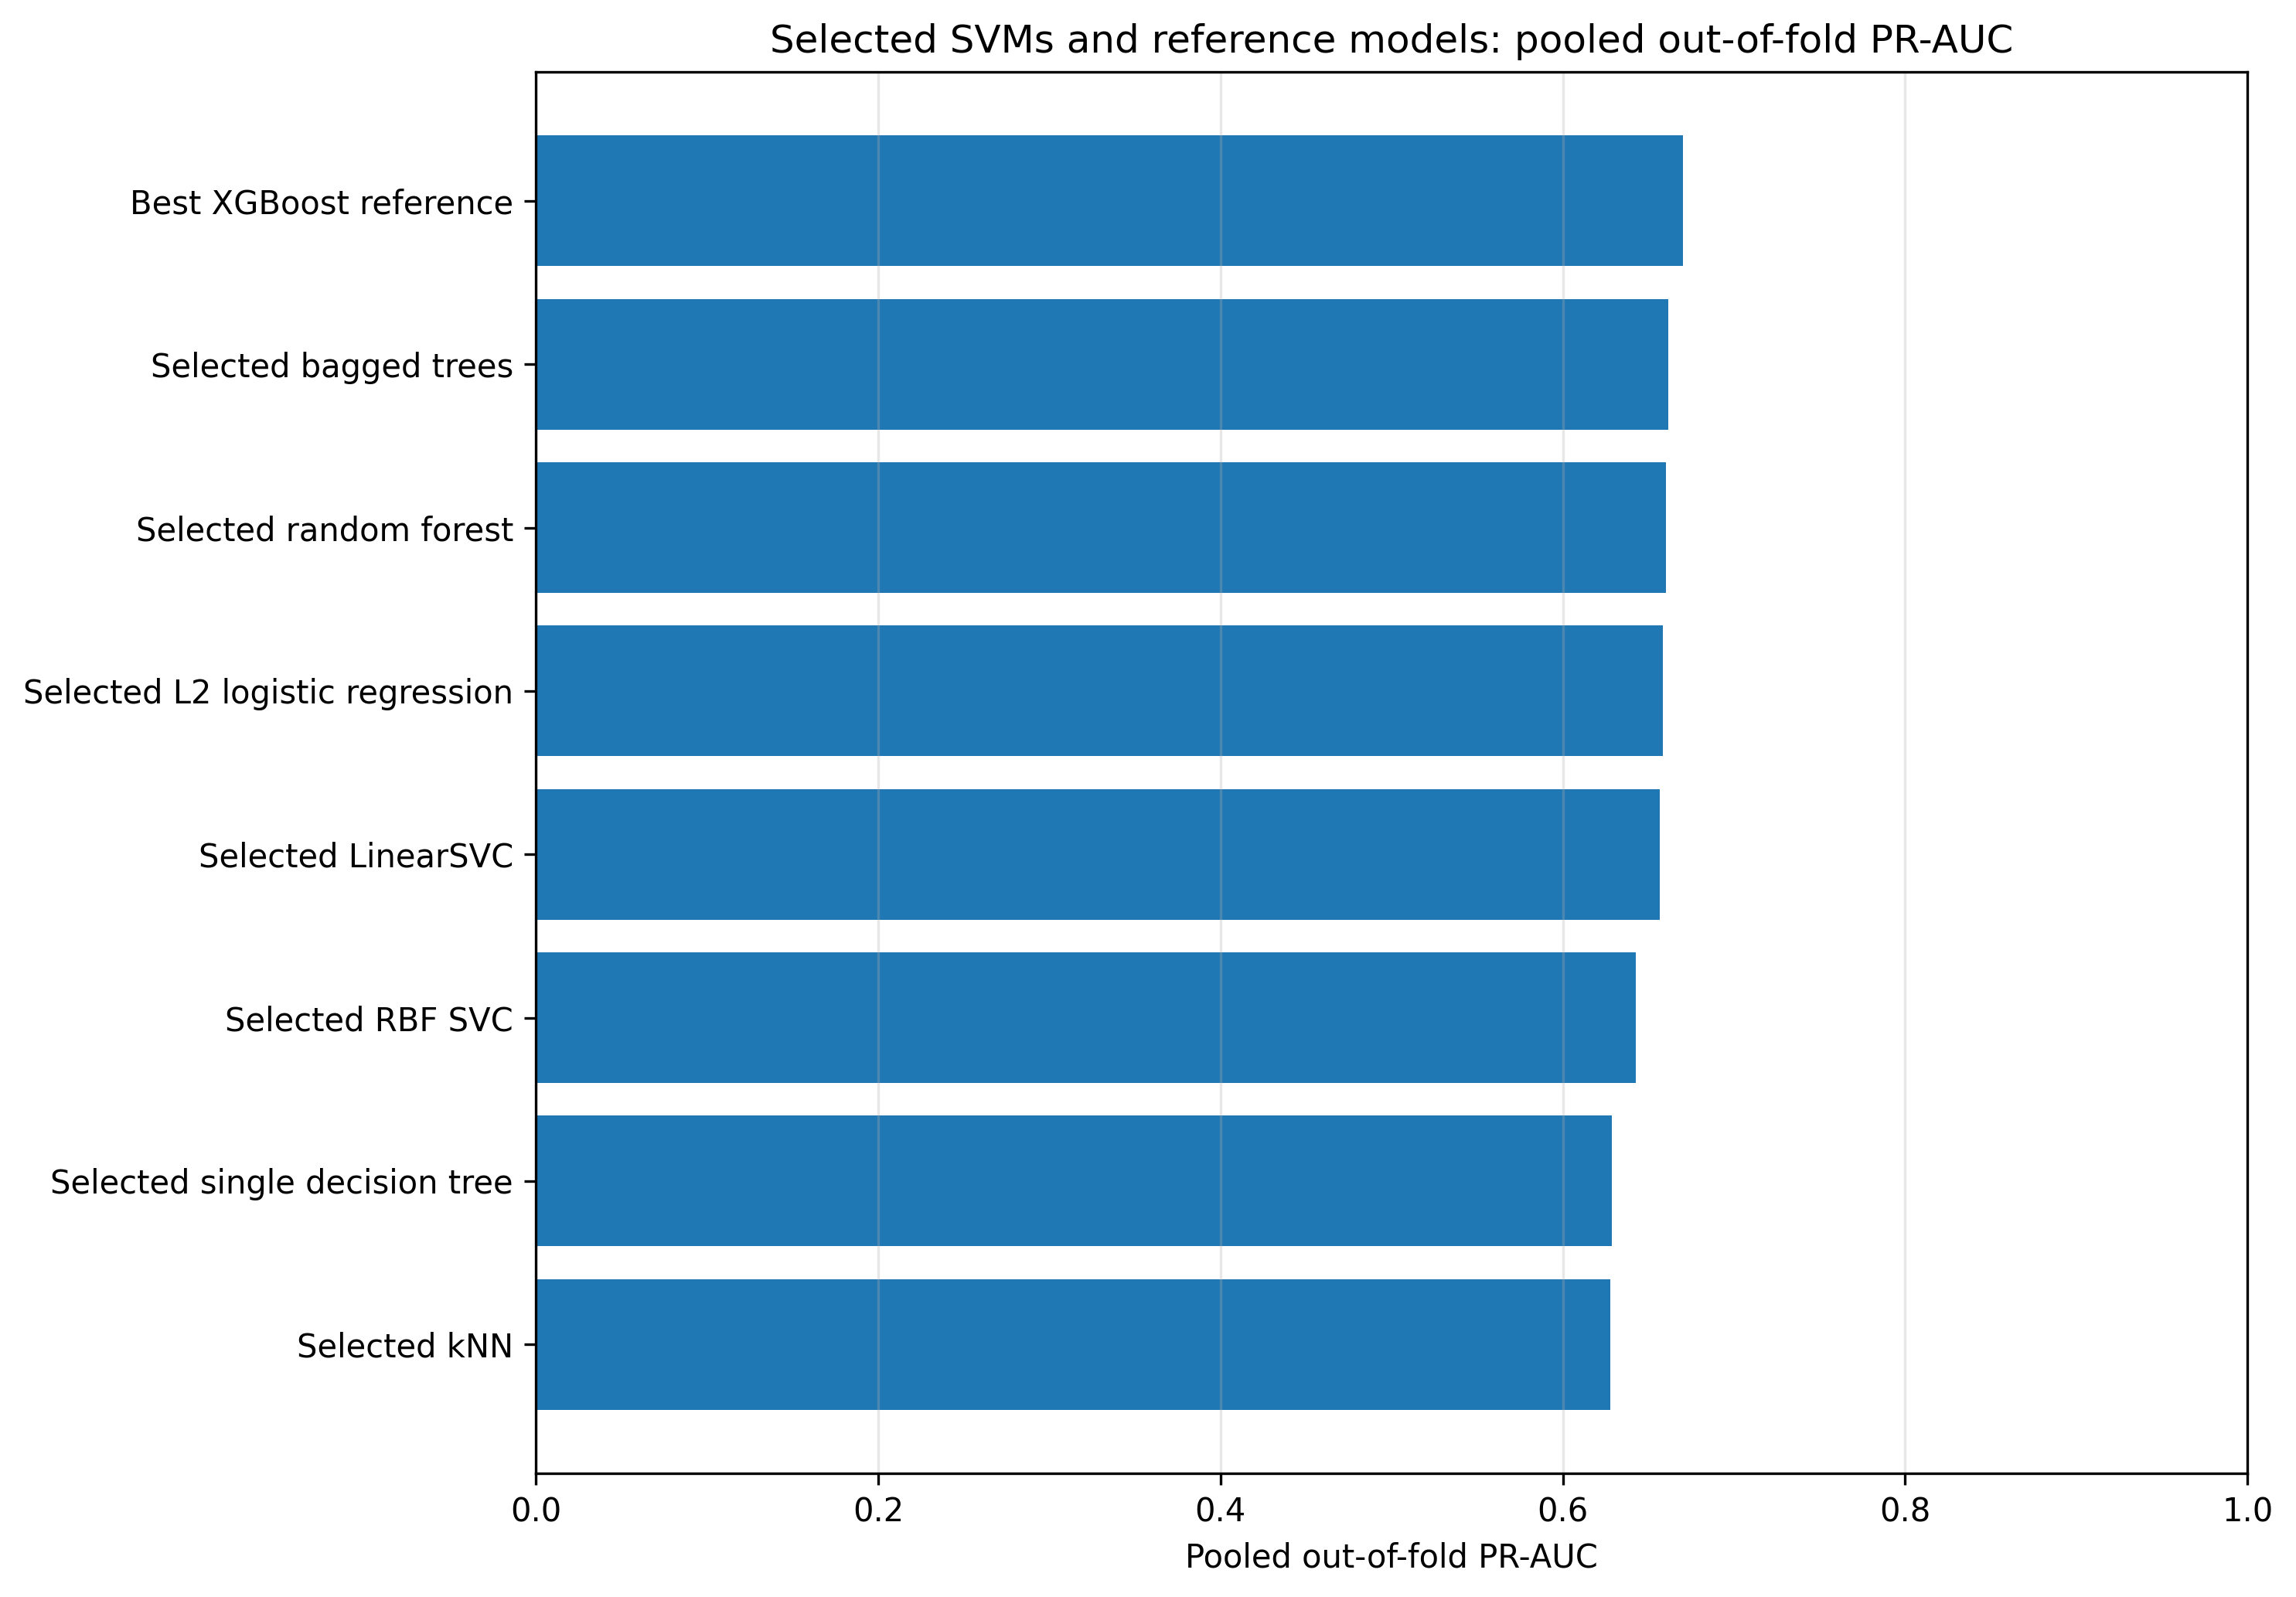
\includegraphics[width=0.88\textwidth]{../figures/svm_model_comparison_pr_auc.png}
\caption{Selected SVMs and scoped reference models: pooled out-of-fold PR-AUC}
\label{fig:svm-model-comparison}
\end{figure}

\subsection{Default-boundary confusion-matrix behaviour}

The selected SVM candidates use the class-weighted default score boundary. Table~\ref{tab:svm-confusion} shows positive-first pooled out-of-fold counts. The selected linear SVM detects \(1206\) of the \(1495\) churners, corresponding to recall \(0.807\), but also produces \(1147\) false positives. The selected RBF SVM detects \(1246\) churners and produces \(1410\) false positives.

\begin{table}[H]
\centering
\small
\begin{tabular}{lrrrrr}
\toprule
Model & TP & FN & FP & TN & Pred. positive rate \\
\midrule
Selected LinearSVC & 1206 & 289 & 1147 & 2992 & 0.418 \\
Selected RBF SVC & 1246 & 249 & 1410 & 2729 & 0.471 \\
Selected L2 logistic regression & 813 & 682 & 434 & 3705 & 0.221 \\
Best XGBoost reference & 806 & 689 & 395 & 3744 & 0.213 \\
\bottomrule
\end{tabular}
\caption{Positive-first pooled out-of-fold confusion-matrix counts for selected SVMs and compact reference models}
\label{tab:svm-confusion}
\end{table}

This default-boundary behaviour follows directly from class weighting. The selected LinearSVC flags approximately \(41.8\%\) of customers as potential churners, compared with an observed churn rate of \(26.5\%\). The classifier therefore prioritizes churn recovery rather than a narrow high-precision intervention list. Whether this is preferable depends on retention capacity and the relative costs of false negatives and false positives.

\subsection{Margin-score threshold behaviour}

The selected linear SVM uses a signed decision score, not a predicted probability. Score \(0\) is the natural SVM boundary. Table~\ref{tab:svm-thresholds} reports selected score thresholds. Lower score thresholds increase recall and reduce precision and specificity. Higher thresholds create a more selective intervention list.

\begin{table}[H]
\centering
\small
\begin{tabular}{rrrrrr}
\toprule
Score threshold & Precision & Recall & Specificity & \(F_1\) & Pred. positive rate \\
\midrule
-0.850 & 0.327 & 0.985 & 0.267 & 0.491 & 0.800 \\
-0.304 & 0.426 & 0.924 & 0.551 & 0.583 & 0.575 \\
0.000 & 0.513 & 0.807 & 0.723 & 0.627 & 0.418 \\
0.135 & 0.561 & 0.740 & 0.791 & 0.638 & 0.350 \\
0.291 & 0.610 & 0.633 & 0.854 & 0.621 & 0.275 \\
0.455 & 0.671 & 0.506 & 0.910 & 0.577 & 0.200 \\
\bottomrule
\end{tabular}
\caption{Margin-score threshold behaviour for the selected LinearSVC using pooled out-of-fold scores}
\label{tab:svm-thresholds}
\end{table}

At the natural score threshold \(0\), the selected linear SVM has precision \(0.513\), recall \(0.807\), specificity \(0.723\), and \(F_1\) \(0.627\). Raising the score threshold to approximately \(0.135\) increases the displayed \(F_1\) to \(0.638\), while lowering recall to \(0.740\). Raising it further to approximately \(0.455\) increases precision to \(0.671\), but recall falls to \(0.506\).

These values should not be used to select a final production threshold in this section. The decision scores are uncalibrated margins, not churn probabilities. A later finalist workflow must connect threshold selection to intervention value, contact capacity, and the relative cost of false negatives and false positives. If probability interpretation becomes necessary, calibration should be assessed as a dedicated training-only step.

\begin{figure}[H]
\centering
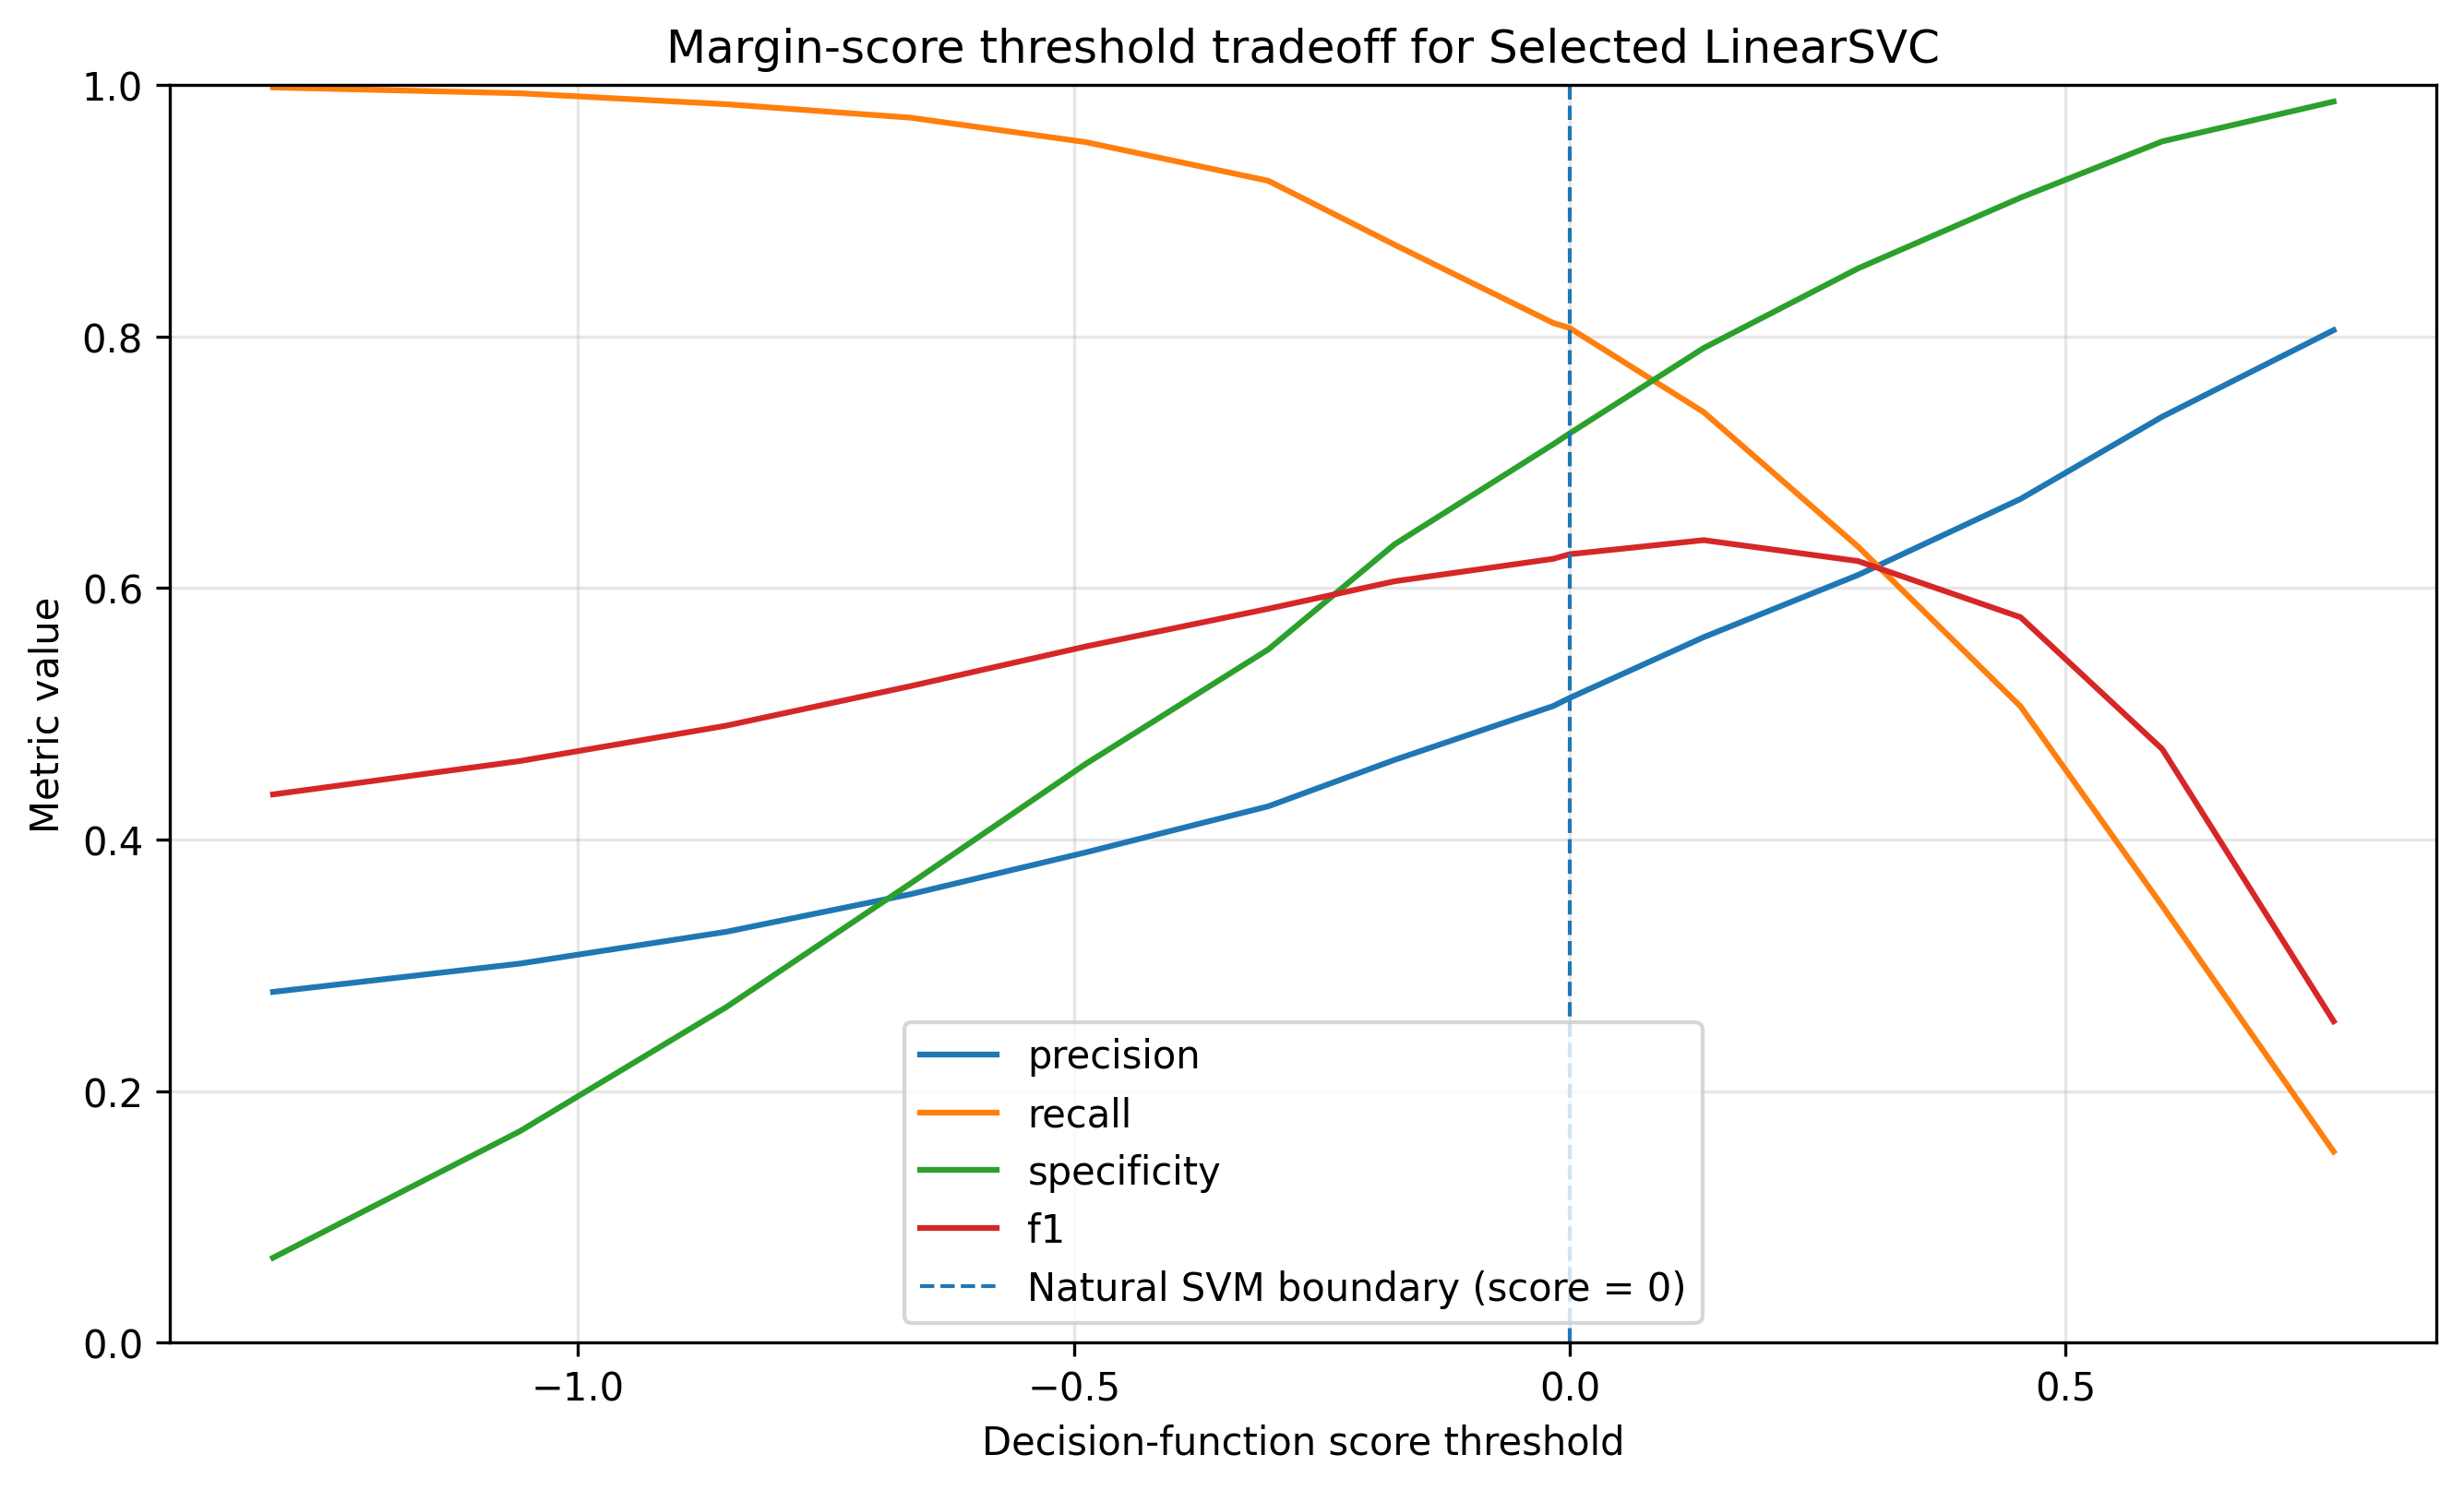
\includegraphics[width=0.88\textwidth]{../figures/svm_margin_score_threshold_tradeoff.png}
\caption{Margin-score threshold tradeoff for the selected LinearSVC}
\label{fig:svm-threshold-tradeoff}
\end{figure}

\subsection{Ranking curves}

Figures~\ref{fig:svm-roc-curve} and~\ref{fig:svm-pr-curve} show the ranking curves for the selected linear SVM. Its pooled OOF ROC-AUC is approximately \(0.845\), while PR-AUC is approximately \(0.657\). The precision-recall curve remains materially above the positive-rate baseline of approximately \(0.265\), indicating that the linear SVM produces useful churn-risk ordering despite the absence of calibrated probabilities.

\begin{figure}[H]
\centering
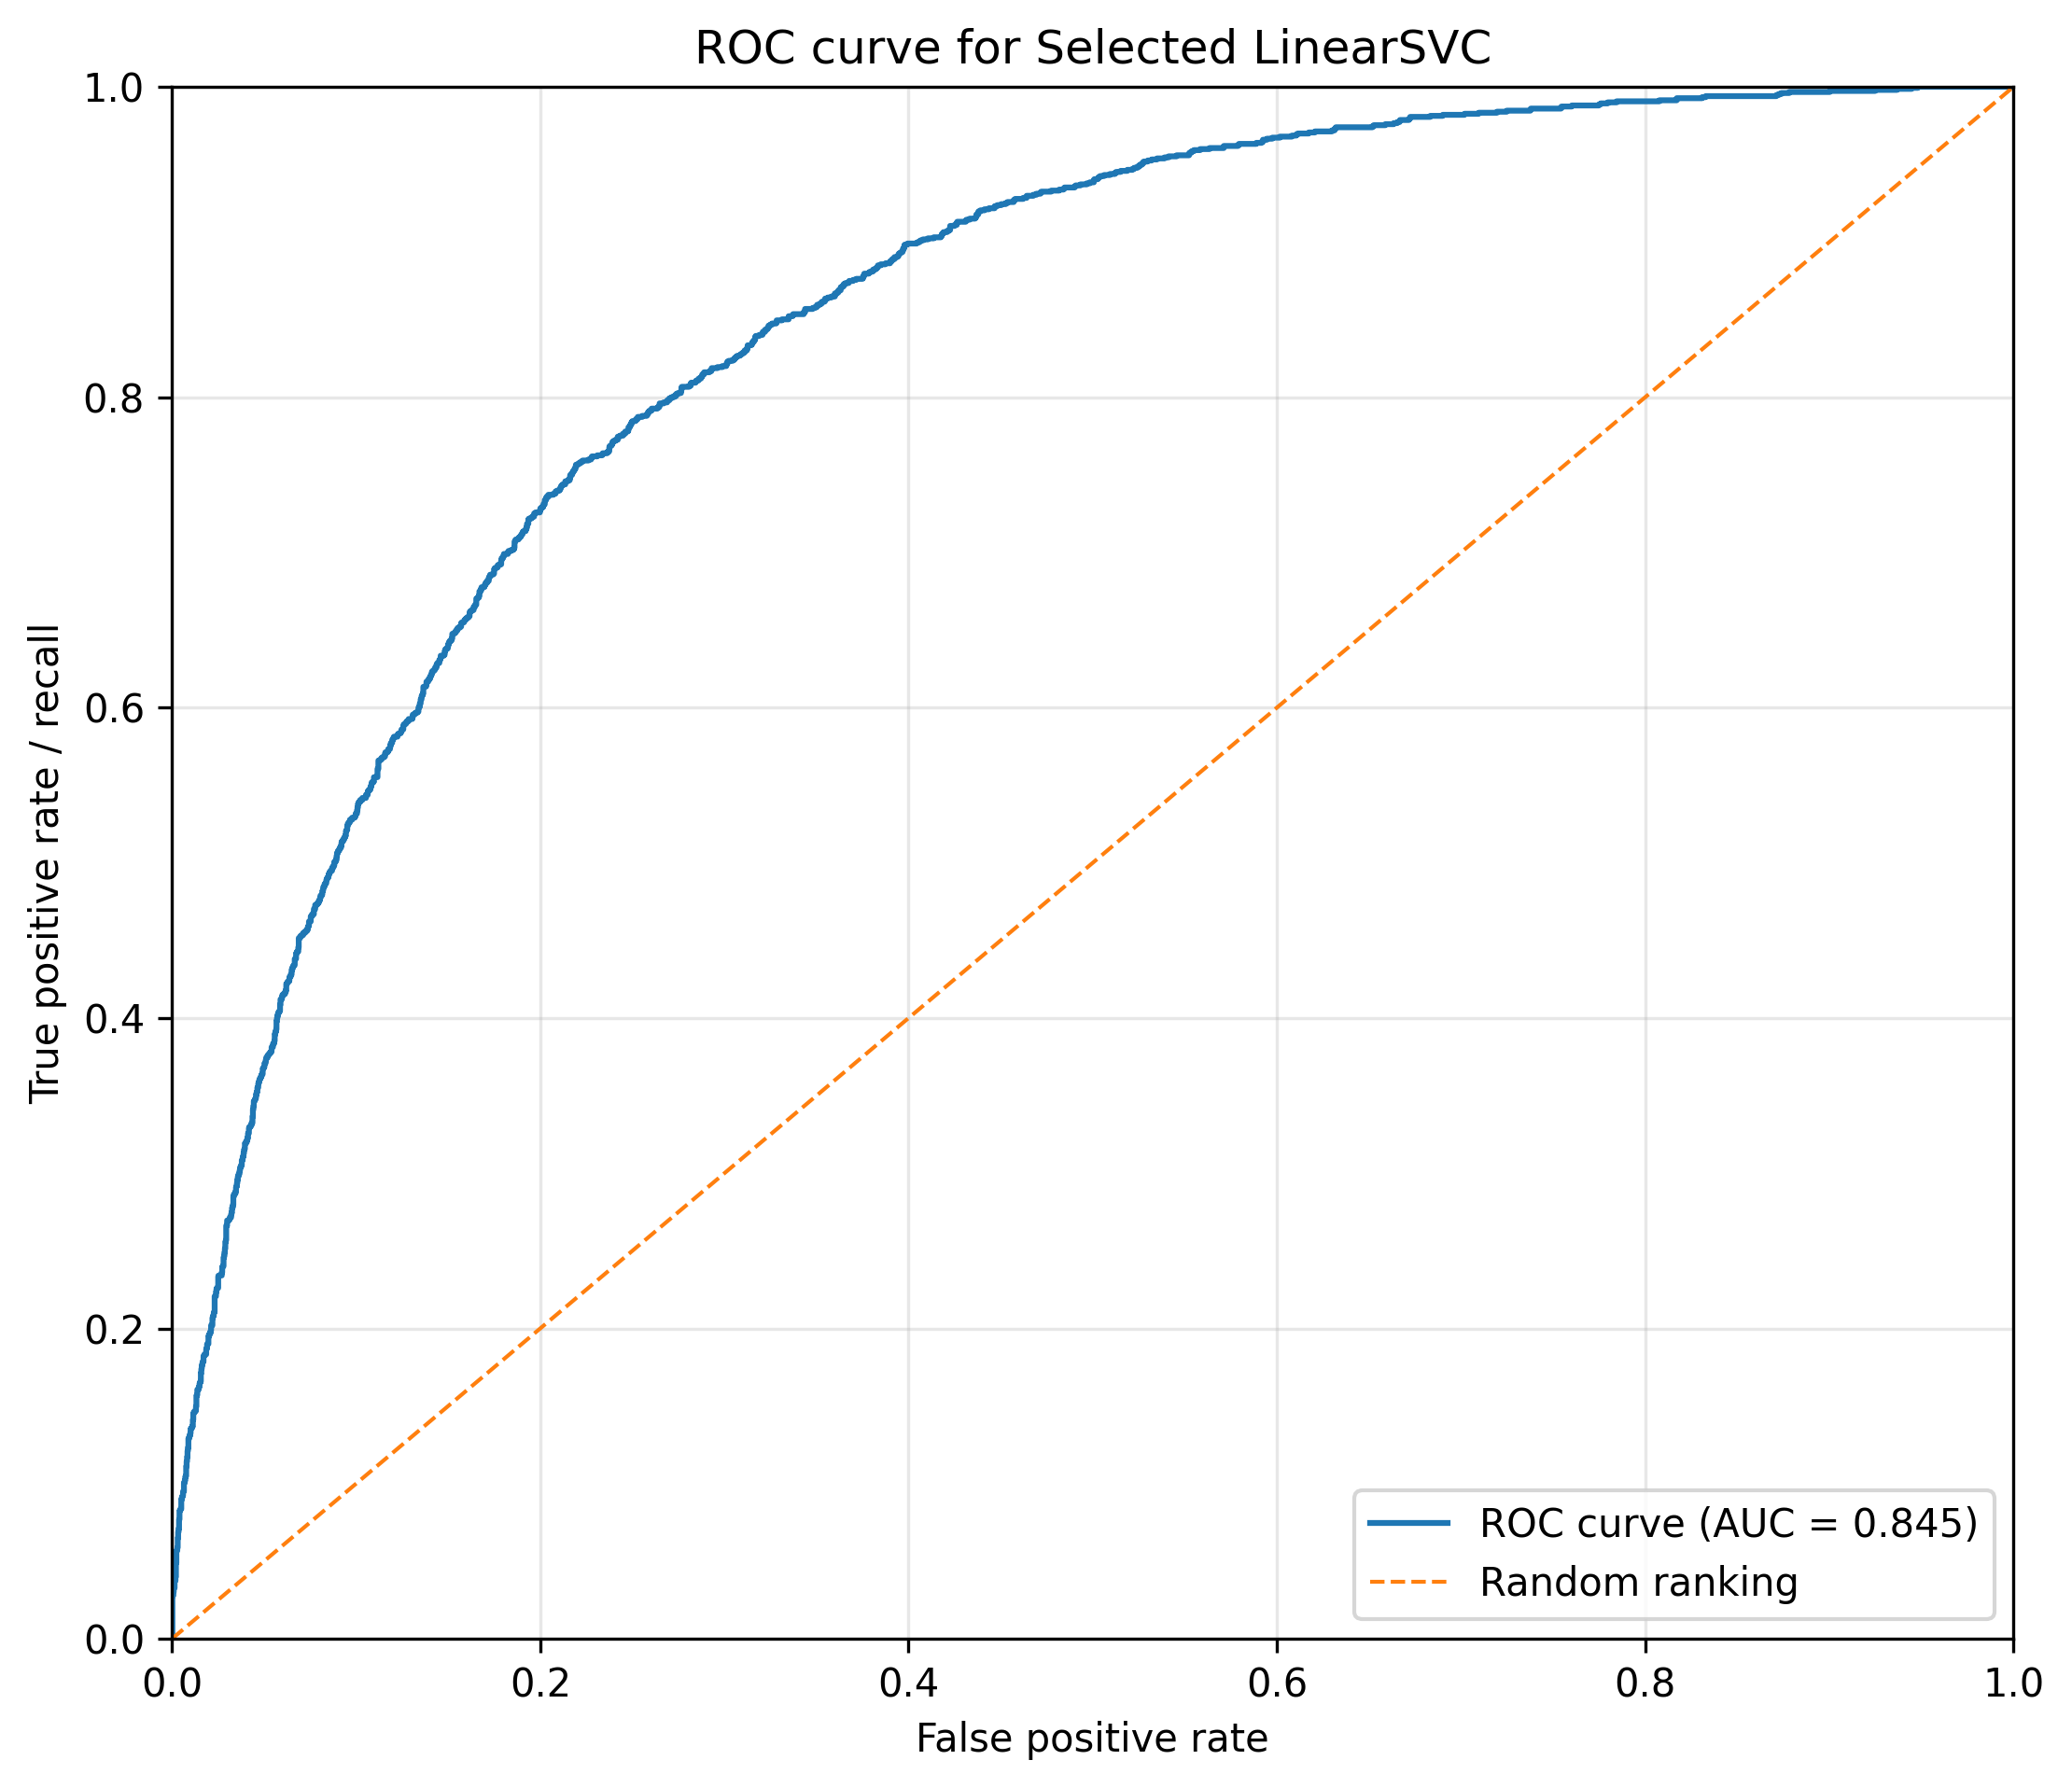
\includegraphics[width=0.82\textwidth]{../figures/svm_roc_curve.png}
\caption{ROC curve for the selected LinearSVC}
\label{fig:svm-roc-curve}
\end{figure}

\begin{figure}[H]
\centering
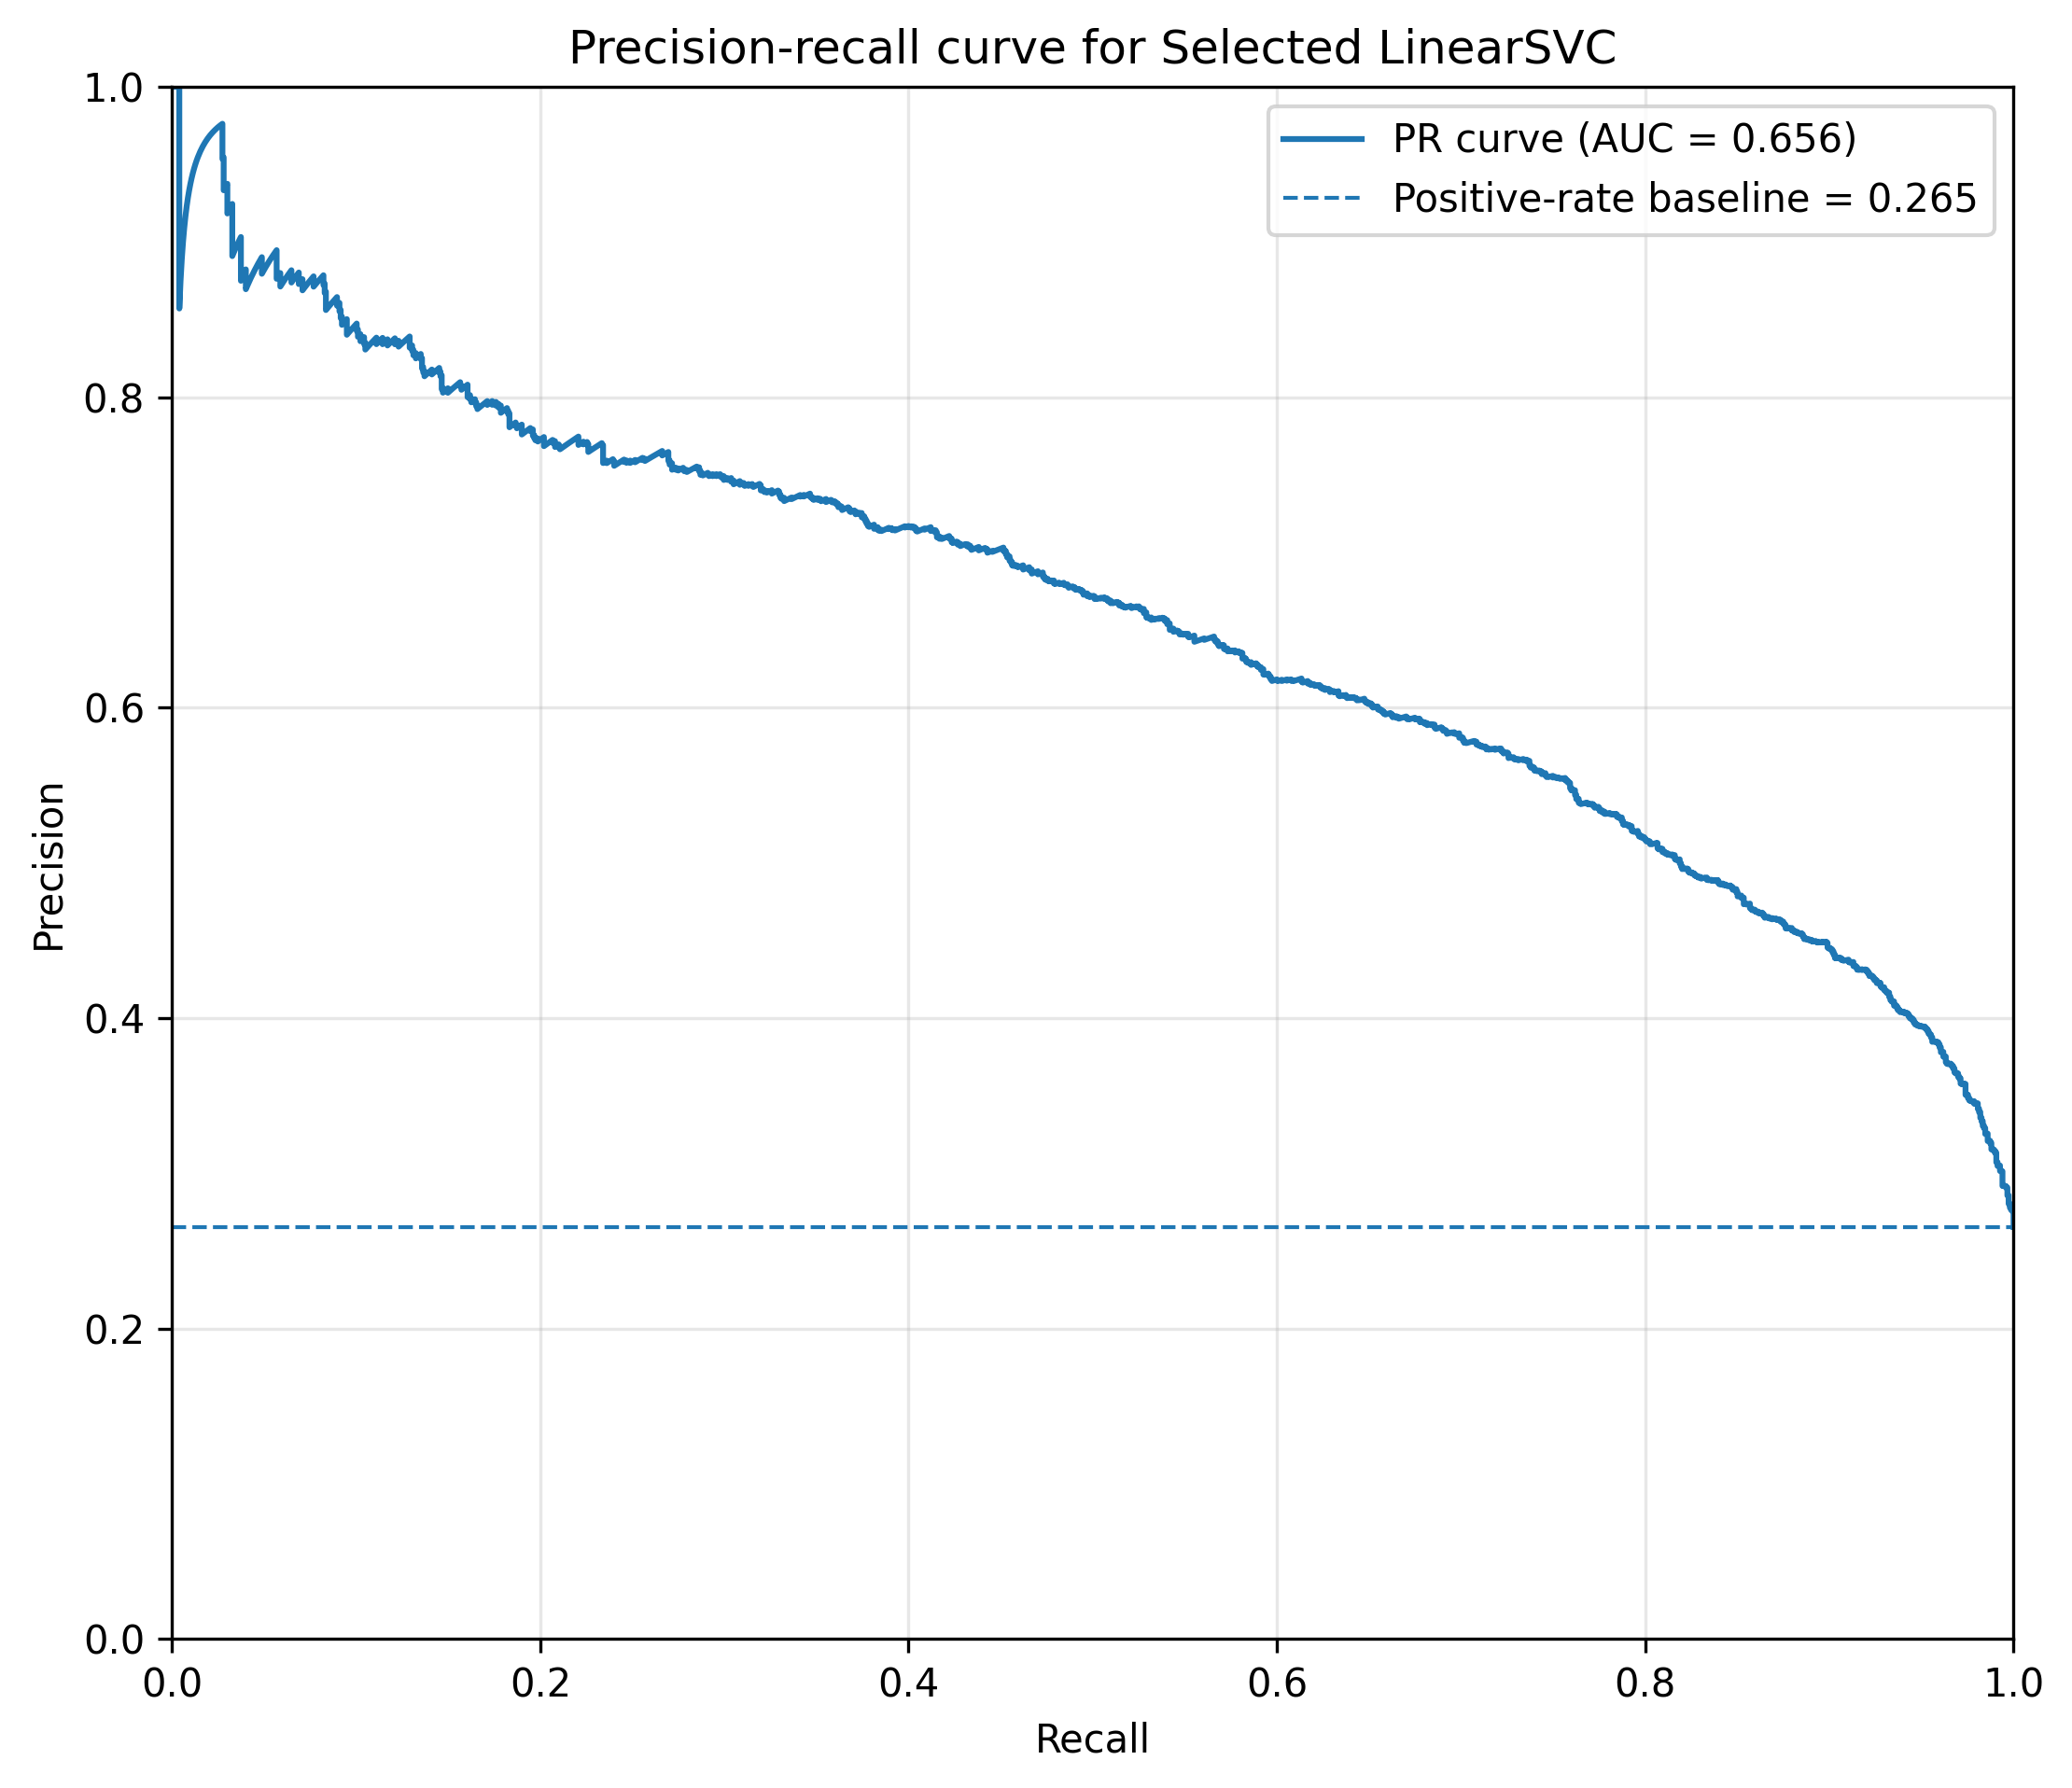
\includegraphics[width=0.82\textwidth]{../figures/svm_precision_recall_curve.png}
\caption{Precision-recall curve for the selected LinearSVC}
\label{fig:svm-pr-curve}
\end{figure}

\subsection{Linear-SVM coefficient directions}

The selected linear SVM is fitted once on the complete training set to inspect coefficient directions. This refit is for interpretation only and does not enter the cross-validated performance estimates. A positive coefficient increases the positive-class SVM decision score, while a negative coefficient decreases it, conditional on the other transformed features.

Table~\ref{tab:svm-linear-coefficients} lists selected large coefficients. The largest positive directions are fiber-optic internet service, month-to-month contract status, streaming services, electronic-check payment, lack of online security, and lack of technical support. The largest negative directions include tenure, DSL service, two-year contract status, and several no-internet-service indicators.

\begin{table}[H]
\centering
\small
\begin{tabular}{lr}
\toprule
Feature & SVM decision-score coefficient \\
\midrule
tenure & -0.322 \\
InternetService\_Fiber optic & 0.279 \\
MonthlyCharges & -0.244 \\
InternetService\_DSL & -0.239 \\
Contract\_Month-to-month & 0.238 \\
Contract\_Two year & -0.223 \\
StreamingMovies\_Yes & 0.107 \\
StreamingTV\_Yes & 0.102 \\
PaymentMethod\_Electronic check & 0.094 \\
OnlineSecurity\_No & 0.083 \\
TechSupport\_No & 0.068 \\
\bottomrule
\end{tabular}
\caption{Selected coefficient directions for the fitted LinearSVC}
\label{tab:svm-linear-coefficients}
\end{table}

\begin{figure}[H]
\centering
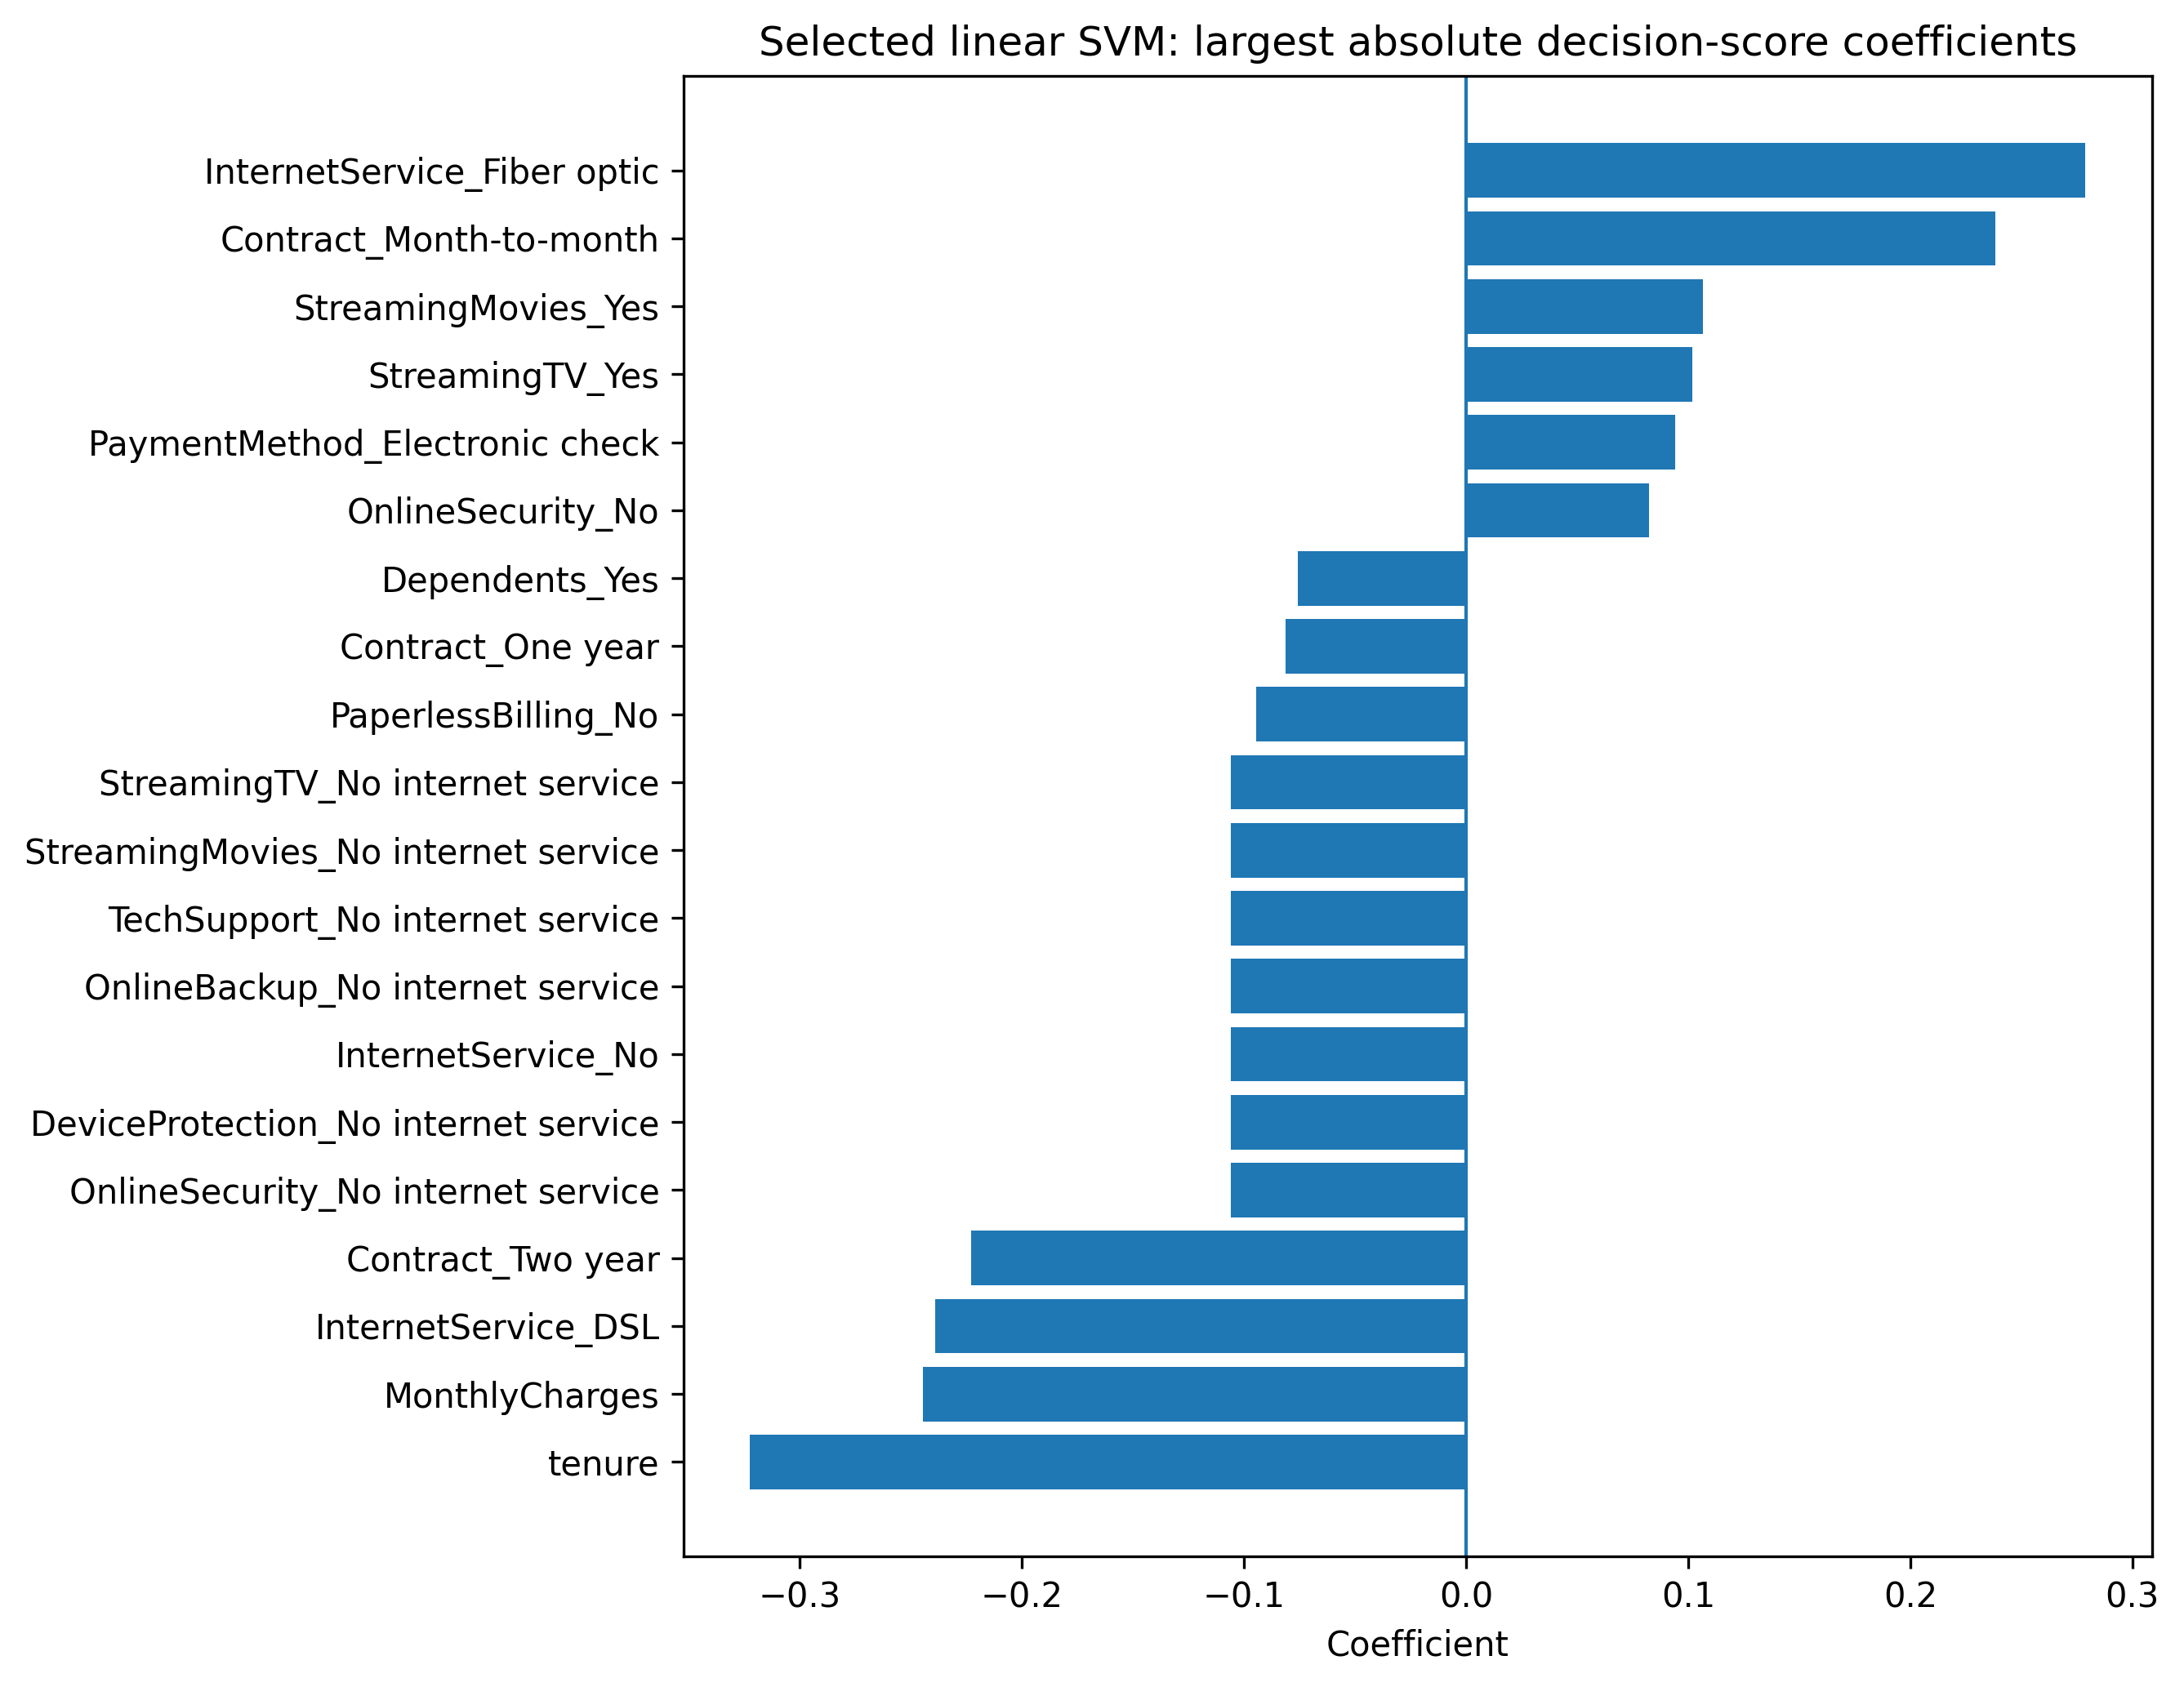
\includegraphics[width=0.84\textwidth]{../figures/svm_linear_coefficients.png}
\caption{Largest absolute decision-score coefficients for the selected LinearSVC}
\label{fig:svm-linear-coefficients}
\end{figure}

The coefficients are not causal effects and are not logistic-regression log-odds coefficients. They must not be exponentiated into odds ratios. They describe how the fitted maximum-margin score changes conditionally within the correlated one-hot encoded representation. In particular, the negative coefficient on \texttt{MonthlyCharges} is conditional on tenure, contract, internet service, and related service features. It should not be interpreted as a marginal statement that higher charges reduce churn.

\subsection{RBF support-vector diagnostic}

The selected RBF SVC is fitted once on the complete training data to summarize its support-vector counts. This is a structural diagnostic only. It does not provide another performance estimate and it does not influence model selection.

\begin{table}[H]
\centering
\small
\begin{tabular}{lrr}
\toprule
Class & Support-vector count & Share of training rows \\
\midrule
Non-churn & 2246 & 0.399 \\
Churn & 816 & 0.145 \\
Total & 3062 & 0.543 \\
\bottomrule
\end{tabular}
\caption{Support-vector diagnostic for the selected RBF SVC fitted on the full training set}
\label{tab:svm-support-vectors}
\end{table}

The selected RBF SVC uses \(3062\) support vectors, equal to approximately \(54.3\%\) of the \(5634\) training observations. A large support-vector share is not inherently problematic, especially in overlapping noisy data. It does show that the nonlinear solution remains structurally more complex than the linear alternative. Because the RBF model does not provide a clear fold-level ranking improvement, this complexity reinforces the preference for the linear SVM as the representative SVM diagnostic model.

\subsection{Section summary}

This section introduced support vector machines as maximum-margin classifiers and evaluated both linear and nonlinear kernel variants. The selected linear configuration uses squared-hinge loss, \(C=0.1\), and balanced class weights. The selected RBF configuration uses \(C=10\), \(\gamma=0.001\), and balanced class weights.

The strongest linear and RBF candidates are effectively tied in mean fold-level validation PR-AUC. The RBF point estimate is only \(0.0001\) higher, far below observed fold-to-fold variation. The kernel-family screen and RBF grid do not demonstrate a material nonlinear advantage, while large \(\gamma\) values show a clear risk of overfitting. The linear SVM is therefore retained as the representative SVM for diagnostics because it is faster, more interpretable, and stronger in the pooled OOF comparison.

The SVM family is competitive with logistic regression and several tree ensembles, but it does not exceed the strongest XGBoost reference in this deliberately scoped comparison. Its class-weighted natural boundary yields high recall at the cost of a substantially larger intervention list. Raw SVM decision scores support ranking and threshold-tradeoff analysis, but they are not calibrated probabilities. A later final training-only comparison will include all serious model-family finalists, define any calibration and threshold procedure, and use the held-out test set exactly once after the complete development policy is fixed.
